\documentclass[12pt, a4paper]{article}

% ==========================================
% 1. KHAI BÁO GÓI THƯ VIỆN (PACKAGES)
% ==========================================
% Bảng mã & Font chữ
\usepackage[utf8]{inputenc}
\usepackage[T5]{fontenc}

% Toán học
\usepackage{amsmath, amssymb}

% Căn lề & Bố cục trang
\usepackage[top=2.2cm, bottom=1.5cm, left=1cm, right=1cm, headheight=15pt]{geometry}
\usepackage{fancyhdr}
\usepackage{needspace}
\usepackage{tkz-tab}

% Đồ họa & Màu sắc
\usepackage{xcolor}
\usepackage{graphicx} 
\usepackage{tikz}
\usetikzlibrary{calc, shapes.geometric, positioning}


% Bảng biểu & Danh sách
\usepackage{colortbl}
\usepackage{array}
\usepackage{makecell}
\usepackage{multirow}
\usepackage{tasks}

% Biểu tượng
\usepackage{fontawesome5}

% ==========================================
% 2. THIẾT LẬP MÀU SẮC CHỦ ĐẠO
% ==========================================
\definecolor{goldyellow}{RGB}{255, 179, 0}
\definecolor{amberorange}{RGB}{230, 115, 0}
\definecolor{lightamber}{RGB}{255, 248, 225}
\definecolor{deepblue}{RGB}{25, 42, 86}
\definecolor{accentred}{RGB}{232, 65, 24}
\definecolor{softgray}{RGB}{220, 220, 222} 
\definecolor{fbblue}{RGB}{15, 80, 200}


% ==========================================
% 3. CẤU HÌNH HEADER & FOOTER
% ==========================================
\pagestyle{fancy}
\fancyhf{}
\renewcommand{\headrulewidth}{0pt}

% Khai báo biến lưu trữ nội dung góc phải của Header
\newcommand{\HeaderRightText}{}

% --- Header ---
\fancyhead[C]{
    \begin{tikzpicture}[remember picture, overlay]
        
        % Dải màu trang trí góc trên
        \path[fill=deepblue] (current page.north west) -- (current page.north east) 
            -- ($(current page.north east) + (0, -1.6cm)$) 
            .. controls ($(current page.north) + (3, -2.0cm)$) and ($(current page.north) + (-3, -0.4cm)$) .. 
            ($(current page.north west) + (0, -1.0cm)$) -- cycle;
            
        \path[fill=goldyellow] (current page.north west) -- (current page.north east) 
            -- ($(current page.north east) + (0, -1.0cm)$) 
            .. controls ($(current page.north) + (4, -1.0cm)$) and ($(current page.north) + (-2, -2.2cm)$) .. 
            ($(current page.north west) + (0, -1.6cm)$) -- cycle;
            
        \path[fill=amberorange] (current page.north west) -- ($(current page.north west) + (6.5cm, 0)$) 
            .. controls ($(current page.north west) + (4.5cm, -1.2cm)$) and ($(current page.north west) + (2cm, -2.0cm)$) .. 
            ($(current page.north west) + (0, -2.0cm)$) -- cycle;
            
        % Logo góc trái Header
        \node[anchor=west, inner sep=0pt] 
            at ($(current page.north west) + (0cm, -0.8cm)$) {
\includegraphics[height=2.0cm]{../../image/logo-header.png}};
            
        % Text góc phải Header (Tự động lấy từ đối số thứ 3 của \titlebox)
        \node[anchor=east, text=white, font=\small\bfseries\sffamily] 
            at ($(current page.north east) + (-0.8cm, -0.5cm)$) {\HeaderRightText};
    \end{tikzpicture}
}

% --- Footer ---
\fancyfoot[C]{
    \begin{tikzpicture}[remember picture, overlay]
        % Đường kẻ ngang
        \draw[amberorange, line width=1.5pt] 
            ($(current page.south west) + (0cm, 0.4cm)$) -- ($(current page.south east) + (0cm, 0.4cm)$);

        % Dải cong góc phải
        \path[fill=goldyellow] (current page.south east) -- ($(current page.south east) + (-5cm, 0)$) 
            .. controls ($(current page.south east) + (-3cm, 0.8cm)$) and ($(current page.south east) + (-1.5cm, 1.2cm)$) .. 
            ($(current page.south east) + (0, 1.2cm)$) -- cycle;

        % Mạng xã hội
        \node[anchor=west, inner sep=0pt] at ($(current page.south west) + (1cm, 0.8cm)$) {
            \small\sffamily
            \textcolor{fbblue}{\faFacebook\hskip 4pt Toán Anh Huy MATH-STER}
            \hskip 18pt
            \textcolor{black}{\faTiktok\hskip 4pt huymathster}
        };

        % Số trang
        \node[circle, fill=white, draw=amberorange, line width=1.5pt, text=deepblue, font=\large\bfseries\sffamily, inner sep=4pt, minimum size=0.8cm] 
            at ($(current page.south east) + (-1.2cm, 0.6cm)$) {\thepage};
    \end{tikzpicture}
}

% ==========================================
% 4. ĐỊNH NGHĨA MACRO: KHUNG TIÊU ĐỀ
% ==========================================
\newcommand{\titlebox}[3]{
    % Gán nội dung đối số #3 vào biến HeaderRightText
    \gdef\HeaderRightText{#3}
    
    \begin{center}
    \vspace*{-0.5cm}
    \begin{tikzpicture}
        % Khung vô hình (Phantom Box) định chuẩn kích thước
        \node[text width=16cm, inner xsep=0pt, inner ysep=16pt, opacity=0] (MainBox) {
            \begin{minipage}[c]{4.2cm}
                \centering\vspace{0.1cm}
                \rule{2.2cm}{2.2cm} 
                \vspace{0.1cm}
            \end{minipage}%
            \begin{minipage}[c]{11.5cm}
                \centering\vspace{0.15cm}
                {\huge\bfseries\sffamily #2 \par}
                \vspace{0.15cm} 
            \end{minipage}
        };
        
        % Đổ bóng & Nền
        \fill[goldyellow, rounded corners=8pt] ([xshift=5pt, yshift=-5pt]MainBox.south west) rectangle ([xshift=5pt, yshift=-5pt]MainBox.north east);
        \fill[white, rounded corners=8pt] (MainBox.south west) rectangle (MainBox.north east);
        
        % Lưới ô ly & Nền Logo
        \begin{scope}
            \clip[rounded corners=8pt] (MainBox.south west) rectangle (MainBox.north east);
            \draw[step=0.4cm, softgray!50, line width=0.6pt] (MainBox.south west) grid (MainBox.north east);
            \fill[lightamber!60] (MainBox.south west) rectangle ([xshift=4.2cm]MainBox.north west);
        \end{scope}

        % Viền ngoài
        \draw[deepblue, line width=1.5pt, rounded corners=8pt] (MainBox.south west) rectangle (MainBox.north east);

        % Nội dung Text (Lớp trên cùng)
        \node[text width=16cm, inner xsep=0pt, inner ysep=16pt] at (MainBox.center) {
            \begin{minipage}[c]{4.2cm}
                \centering
                % --- ĐIỀU CHỈNH TỌA ĐỘ LOGO Ở ĐÂY ---
                \hspace*{-0.5cm}\raisebox{-0.2cm}{
\includegraphics[width=5.5cm]{../../image/logo.png}}
            \end{minipage}%
            \begin{minipage}[c]{11.5cm}
                \centering\vspace{0.15cm}
                {\huge\bfseries\sffamily\color{deepblue} #2 \par}
                \vspace{0.15cm} 
            \end{minipage}
        };
        
        % Trang trí phụ kiện
        \draw[deepblue, line width=1.5pt, dashed] ([xshift=4.2cm]MainBox.north west) -- ([xshift=4.2cm]MainBox.south west);
        \node[regular polygon, regular polygon sides=4, rotate=45, fill=white, draw=accentred, line width=1.2pt, inner sep=2.5pt] at ([xshift=4.2cm]MainBox.west) {};
        \node[anchor=west, fill=amberorange, text=white, font=\large\bfseries\sffamily, rounded corners=4pt, draw=deepblue, line width=1.5pt, inner xsep=12pt, inner ysep=6pt] at ([xshift=1.5cm]MainBox.north west) {#1};
        \fill[accentred] ([xshift=-1.8cm, yshift=-0.4cm]MainBox.north east) circle (3pt);
        \fill[amberorange] ([xshift=-1.4cm, yshift=-0.4cm]MainBox.north east) circle (3pt);
        \fill[goldyellow] ([xshift=-1.0cm, yshift=-0.4cm]MainBox.north east) circle (3pt);
    \end{tikzpicture}
    \vspace*{0cm}
    \end{center}
}

% ==========================================
% 5. ĐỊNH NGHĨA MACRO: CẤU TRÚC CÂU HỎI (ÉP SÁT NHAU)
% ==========================================
\newcommand{\questioncore}[2]{
    % Xóa khoảng cách phía trên, ép sát câu trước
    \noindent \textbf{\textcolor{deepblue}{Câu #1.} \textcolor{accentred}{[STER]}} #2
    \par\nopagebreak
}

% Cấu hình hiển thị đáp án trắc nghiệm
\settasks{
    label=\textbf{\textcolor{amberorange}{\Alph*.}}, 
    label-width=15pt,     
    item-indent=25pt,     
    label-offset=6pt,    
    column-sep=20pt,     
    after-item-skip=2pt  % Đã giảm tối đa khoảng cách giữa các dòng đáp án A B C D
}

% Hàm vẽ dòng kẻ nháp
\newcommand{\drawdashlines}[1]{
    \ifnum#1>0
        \nopagebreak\vspace{0.1cm}\noindent 
        \begin{tikzpicture}
            \foreach \i in {1,...,#1} {
                \draw[softgray, line width=0.2pt] (0,-{\i*0.65}) -- (\textwidth-4pt,-{\i*0.65});
            }
        \end{tikzpicture}
        \par
    \fi
    % Đã xóa hoàn toàn khoảng cách thừa ở nhánh else
}

% --- Dạng 1: Trắc nghiệm 4 đáp án ---
\newcommand{\questionLinesManual}[4]{
    \pgfmathsetmacro{\calculatedSpace}{1.5 + #1 * 0.65}
    \needspace{\calculatedSpace cm} 
    \questioncore{#2}{#3}
    #4
    \par\nopagebreak
    \drawdashlines{#1}
}

% --- Dạng 2: Trắc nghiệm Đúng/Sai ---
\newcommand{\questionTrueFalse}[4]{
    \pgfmathsetmacro{\calculatedSpace}{3.0 + #1 * 0.65} 
    \needspace{\calculatedSpace cm}
    \questioncore{#2}{#3}
    
    \nopagebreak
    \begin{center}
    \renewcommand{\arraystretch}{1.2} % Bóp nhỏ chiều cao của bảng Đ/S
    \begin{tabular}{|>{\centering\arraybackslash}m{0.8cm}|m{12cm}|>{\centering\arraybackslash}m{2cm}|>{\centering\arraybackslash}m{2cm}|}
        \hline
        \rowcolor{amberorange!20}
        & \multicolumn{1}{>{\centering\arraybackslash}m{12cm}|}{\textbf{\textcolor{deepblue}{Mệnh đề}}} & 
        \textbf{\textcolor{deepblue}{Đúng}} & 
        \textbf{\textcolor{deepblue}{Sai}} \\
        \hline
        #4
        \hline
    \end{tabular}
    \renewcommand{\arraystretch}{1}
    \end{center}
    
    \par\nopagebreak
    \drawdashlines{#1}
}

% ----- Dạng 3: Tự luận ngắn -----
\newcommand{\questionShortAnswer}[3]{
    \pgfmathsetmacro{\calculatedSpace}{1.5 + #1 * 0.8}
    \needspace{\calculatedSpace cm}
    
    {\linespread{1.1}\selectfont % Bóp nhỏ giãn dòng của câu tự luận
    \questioncore{#2}{#3}\par}
    
    \nopagebreak
    \begin{flushright}
        \begin{tikzpicture}
            \node[anchor=east, font=\small\bfseries\sffamily, text=deepblue] 
                at (-0.2, 0.4) {Đáp án:};
            \fill[goldyellow, rounded corners=3pt] (0.08, -0.08) rectangle (3.08, 0.72);
            \draw[draw=deepblue, fill=white, line width=1.2pt, rounded corners=3pt] 
                (0,0) rectangle (3.0, 0.8);
            \foreach \x in {0.75, 1.5, 2.25} {
                \draw[draw=deepblue, line width=0.6pt] (\x, 0) -- (\x, 0.8);
            }
        \end{tikzpicture}
    \end{flushright}
    
    \par\nopagebreak
    \drawdashlines{#1}
}

% ==========================================
% BẮT ĐẦU NỘI DUNG TÀI LIỆU
% ==========================================
\begin{document}

% Truyền 3 tham số: {Nhãn cam} {Chữ to chính giữa} {Chữ ở góc phải Header}
\titlebox{Chủ đề: Hàm số}{Giá trị lớn nhất - giá trị nhỏ nhất}{Hàm số: GTLN - GTNN}

% --- CÂU 1: ĐỒ THỊ HÀM SỐ TRÊN ĐOẠN [-3;5] ---
\questionLinesManual{0}{1}{ Cho hàm số \( y = f(x) \) liên tục trên đoạn \([-3; 5]\) và có đồ thị như hình vẽ. Giá trị lớn nhất của hàm số \( y = f(x) \) trên đoạn \([-3; 5]\) bằng

\begin{center}
\begin{tikzpicture}[>=latex, scale=0.8]
    % 1. Vẽ hệ trục tọa độ Ox, O
    \draw[->] (-4,0) -- (5.5,0) node[below] {\small $x$};
    \draw[->] (0,-3) -- (0,4.5) node[right] {\small $y$};
    \node[below left] at (0,0) {\small $O$};
    
    % 2. Vẽ đồ thị hàm số (dạng sóng)
    \draw[thick, color=black!80, samples=150, domain=-3.5:1] 
       plot (\x, {\x + 1});
    \draw[thick, color=black!80, samples=150, domain=1:5]    
        plot (\x, {3/8*\x*\x - 2*\x + 29/8});   
    % 3. Đánh dấu các điểm
    \draw[dashed] (0,-2) -- (-3,-2) -- (-3,0);
    \draw[dashed] (3,0) -- (3,1) -- (0,1);
     \draw[dashed] (1,0) -- (1,2) -- (0,2);
    \draw[dashed] (5,0) -- (5,3) -- (0,3);
    \node[below] at (-3,0) {\small $-3$};
    \node[below] at (5,0) {\small $5$};
    \node[left] at (0,3) {\small $3$};
    \node[left] at (0,2) {\small $2$};
    \node[left] at (0,1) {\small $1$};
    \node[right] at (0,-2) {\small $-2$};
    \node[below] at (-1,0) {\small $-1$};
    \node[below] at (1,0) {\small $1$};
    \node[below] at (3,0) {\small $3$};
\end{tikzpicture}
\end{center}

}{
    \begin{tasks}(4)
        \task 3
        \task 5
        \task $-3$
        \task 2
    \end{tasks}
}

% --- CÂU 2: ĐỒ THỊ HÀM SỐ TRÊN ĐOẠN [-2;4] ---
\questionLinesManual{0}{2}{ Cho hàm số \( y = f(x) \) xác định trên \([-2; 4]\) có đồ thị như hình vẽ bên. Giá trị lớn nhất hàm số \( y = f(x) \) trên đoạn \([0; 4]\) là

\begin{center}
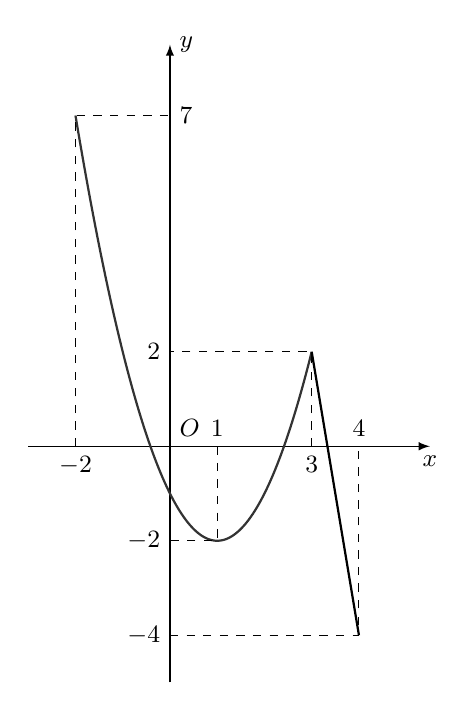
\begin{tikzpicture}[>=latex, scale=0.6]
    % 1. Vẽ hệ trục tọa độ Ox, Oy
    \draw[->] (-3,0) -- (5.5,0) node[below] {\small $x$};
    \draw[->] (0,-5) -- (0,8.5) node[right] {\small $y$};
    \node[above right] at (0,0) {\small $O$};
    
    % 2. Vẽ đồ thị hàm số (dạng đa thức bậc 3)
    \draw[thick, color=black!80, samples=150, domain=-2:3] 
        plot (\x, {\x*\x - 2*\x - 1});
    \draw[thick] (3,2) -- (4,-4);
    % 3. Đánh dấu các điểm
    \draw[dashed] (0,-4) -- (4,-4) -- (4,0);
    \draw[dashed] (1,0) -- (1,-2) -- (0,-2);
    \draw[dashed] (3,0) -- (3,2) -- (0,2);
    \draw[dashed] ( -2,0) -- (-2,7) -- (0,7);
    \node[above] at (4,0) {\small $4$};
    \node[left] at (0,-4) {\small $-4$};
    \node[right] at (0,7) {\small $7$};
    \node[left] at (0,-2) {\small $-2$};
    \node[left] at (0,2) {\small $2$};
    % Đánh dấu các mốc trên trục Ox
    \node[below] at (-2,0) {\small $-2$};
    \node[above] at (1,0) {\small $1$};
    \node[below] at (3,0) {\small $3$};
\end{tikzpicture}
\end{center}

}{
    \begin{tasks}(4)
        \task 3
        \task 2
        \task $-2$
        \task 7
    \end{tasks}
}

% --- CÂU 3: ĐỒ THỊ HÀM SỐ TRÊN KHOẢNG (-∞; -1) ---
\questionLinesManual{0}{3}{ Cho hàm số \( f(x) \) có đồ thị như hình vẽ

\begin{center}
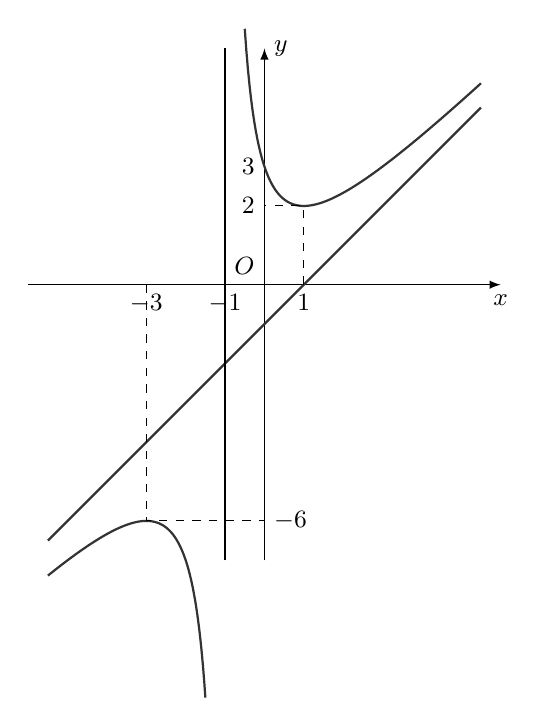
\begin{tikzpicture}[>=latex, scale=0.5]
    % 1. Vẽ hệ trục tọa độ Ox, Oy
    \draw[->] (-6,0) -- (6,0) node[below] {\small $x$};
    \draw[->] (0,-7) -- (0,6) node[right] {\small $y$};
    \node[above left] at (0,0) {\small $O$};
    
    % 2. Vẽ đồ thị hàm số (dạng bậc 3)
    \draw[thick, color=black!80, samples=150, domain=-5.5:-1.5] 
        plot (\x, {(\x*\x + 3)/(\x + 1)});
    \draw[thick, color=black!80, samples=150, domain=-0.5:5.5] 
        plot (\x, {(\x*\x + 3)/(\x + 1)});
    \draw[thick, color=black!80, samples=150, domain=-5.5:5.5]
        plot (\x, {\x - 1});
    % 3. Đánh dấu các điểm
    \draw[dashed] (-3,0) -- (-3,-6) -- (0,-6);
    \draw[dashed] (1,0) -- (1,2) -- (0,2);
    \node[below] at (-1,0) {\small $-1$};
    \node[right] at (0,-6) {\small $-6$};
    \node[left] at (0,3) {\small $3$};
    \node[left] at (0,2) {\small $2$};
    
    % Đánh dấu các mốc trên trục Ox
    \node[below] at (-3,0) {\small $-3$};
    \node[below] at (1,0) {\small $1$};
    \draw[thick] (-1,-7) -- (-1,6);
\end{tikzpicture}
\end{center}

Giá trị lớn nhất của hàm số đã cho trên khoảng \((-\infty; -1)\) bằng}{
    \begin{tasks}(4)
        \task 1
        \task 2
        \task $-6$
        \task $-3$
    \end{tasks}
}



% --- CÂU 4 (tương ứng Câu 13 gốc: THPT Triệu Sơn 4) ---
\questionLinesManual{0}{4}{ Cho hàm số \( y = f(x) \) liên tục và có đồ thị trên đoạn \([-2; 4]\) như hình vẽ bên. Tổng giá trị lớn nhất và nhỏ nhất của hàm số \( y = f(x) \) trên đoạn \([-2; 4]\) bằng

\begin{center}
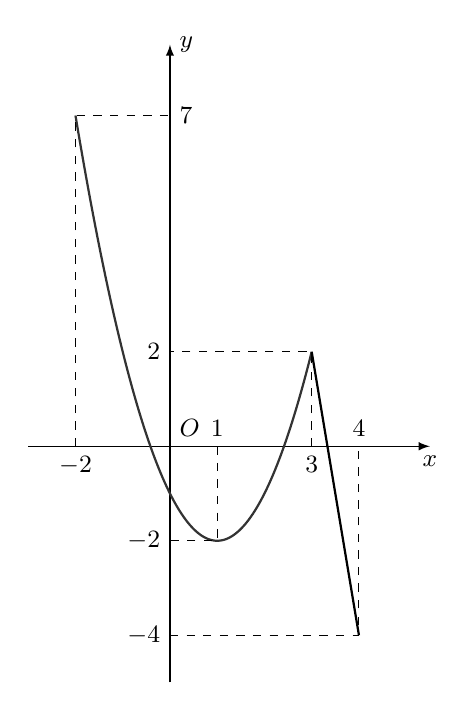
\begin{tikzpicture}[>=latex, scale=0.6]
    % 1. Vẽ hệ trục tọa độ Ox, Oy
    \draw[->] (-3,0) -- (5.5,0) node[below] {\small $x$};
    \draw[->] (0,-5) -- (0,8.5) node[right] {\small $y$};
    \node[above right] at (0,0) {\small $O$};
    
    % 2. Vẽ đồ thị hàm số (dạng đa thức bậc 3)
    \draw[thick, color=black!80, samples=150, domain=-2:3] 
        plot (\x, {\x*\x - 2*\x - 1});
    \draw[thick] (3,2) -- (4,-4);
    % 3. Đánh dấu các điểm
    \draw[dashed] (0,-4) -- (4,-4) -- (4,0);
    \draw[dashed] (1,0) -- (1,-2) -- (0,-2);
    \draw[dashed] (3,0) -- (3,2) -- (0,2);
    \draw[dashed] ( -2,0) -- (-2,7) -- (0,7);
    \node[above] at (4,0) {\small $4$};
    \node[left] at (0,-4) {\small $-4$};
    \node[right] at (0,7) {\small $7$};
    \node[left] at (0,-2) {\small $-2$};
    \node[left] at (0,2) {\small $2$};
    % Đánh dấu các mốc trên trục Ox
    \node[below] at (-2,0) {\small $-2$};
    \node[above] at (1,0) {\small $1$};
    \node[below] at (3,0) {\small $3$};
\end{tikzpicture}
\end{center}

}{
    \begin{tasks}(4)
        \task $-2$
        \task $5$
        \task $3$
        \task $0$
    \end{tasks}
}

% --- CÂU 5 (tương ứng Câu 17 gốc: Sở Văn Phúc) ---
\questionLinesManual{0}{5}{Cho hàm số \( y = f(x) \) liên tục trên đoạn \([-2; 6]\) và có đồ thị như hình vẽ sau. Tổng giá trị lớn nhất và giá trị nhỏ nhất của hàm số \( y = f(x) \) trên đoạn \([-2; 6]\) bằng

\begin{center}
\begin{tikzpicture}[>=latex, scale=0.8]
    % 1. Vẽ hệ trục tọa độ Ox, Oy
    \draw[->] (-3,0) -- (7,0) node[below] {\small $x$};
    \draw[->] (0,-5) -- (0,6) node[left] {\small $y$};
    \node[above left] at (0,0) {\small $O$};
    
    % Ký hiệu vuông góc tại gốc tọa độ (nếu cần giống hình)
    \draw (0,0.2) -- (0.2,0.2) -- (0.2,0);

    % 2. Vẽ đồ thị hàm số y = f(x) chia làm các nhánh:
    % Nhánh 1: Đoạn thẳng từ (-2, -1) đến (-1, 0)
    \draw[thick] (-2,-1) -- (-1,0);
    
    \draw[thick, samples=150, domain=-1:4] plot (\x, {\x*\x - 2*\x - 3});
    
    % Nhánh 3: Đoạn thẳng nằm ngang từ (4, 5) đến (6, 5)
    \draw[thick] (4,5) -- (6,5);
    
    % Tên đồ thị
    \node[right] at (3.2,-2) {\small $y = f(x)$};

    % 3. Vẽ các đường nét đứt và điền số trục tọa độ
    % Tại x = -2, y = -1
    \draw[dashed] (-2,0) -- (-2,-1) -- (0,-1);
    \node[above] at (-2,0) {\small $-2$};
    \node[above] at (-1,0) {\small $-1$};
    \node[right] at (0,-1) {\small $-1$};
    
    % Tại x = 0, y = -3
    \node[left] at (0,-3) {\small $-3$};
    
    % Tại x = 1, y = -4
    \draw[dashed] (1,0) -- (1,-4) -- (0,-4);
    \node[above] at (1,0) {\small $1$};
    \node[left] at (0,-4) {\small $-4$};
    
    % Giao điểm x = 3
    \node[below right] at (3,0) {\small $3$};
    
    % Tại x = 4, y = 5
    \draw[dashed] (4,0) -- (4,5) -- (0,5);
    \node[below] at (4,0) {\small $4$};
    \node[left] at (0,5) {\small $5$};
    
    % Tại x = 6
    \draw[dashed] (6,0) -- (6,5);
    \node[below] at (6,0) {\small $6$};

\end{tikzpicture}
\end{center}

}{
    \begin{tasks}(4)
        \task $1$
        \task $5$
        \task $4$
        \task $2$
    \end{tasks}
}

% --- CÂU 6 (tương ứng Câu 21 gốc: THPT Trần Nguyên Hãn) ---
\questionLinesManual{0}{6}{ Cho hàm số \( y = f(x) \) liên tục trên \([-1; 3]\) và có đồ thị như hình bên.

\begin{center}
\begin{tikzpicture}[>=latex, scale=0.8]
    % 1. Hệ trục tọa độ Ox, Oy
    \draw[->] (-2.5,0) -- (4.5,0) node[below] {\small $x$};
    \draw[->] (0,-5) -- (0,3) node[left] {\small $y$};
    \node[below left] at (0,0) {\small $O$};
    
    % 2. Đồ thị hàm số từng nhánh
    % Nhánh 1: Parabol từ x = -1 (y = 2) qua y-intercept (0, -3) đến cực đại (1, -2)
    % Hàm mẫu phù hợp: y = x^3 - 3x - 3 (độ dốc cong mượt) hoặc dùng cubic bezier
    \draw[thick, samples=100, domain=-1:1]  plot (\x, {-2*\x*\x*\x + 3*\x*\x - 3});
    
    % Nhánh 2: Đoạn thẳng từ (1, -2) xuống (2, -4)
    \draw[thick] (1,-2) -- (2,-4);
    
    % Nhánh 3: Đoạn thẳng từ (2, -4) lên (3, 1)
    \draw[thick] (2,-4) -- (3,1);

    % 3. Đường nét đứt và các mốc tọa độ
    % Tại x = -1, y = 2
    \draw[dashed] (-1,0) -- (-1,2) -- (0,2);
    \node[below left] at (-1,0) {\small $-1$};
    \node[right] at (0,2) {\small $2$};
    
    % Tại x = 0, y = -3 và y = 1
    \node[left] at (0,-3) {\small $-3$};
    \node[left] at (0,1) {\small $1$};
    
    % Tại x = 1, y = -2
    \draw[dashed] (1,0) -- (1,-2) -- (0,-2);
    \node[above] at (1,0) {\small $1$};
    \node[left] at (0,-2) {\small $-2$};
    
    % Tại x = 2, y = -4
    \draw[dashed] (2,0) -- (2,-4) -- (0,-4);
    \node[above] at (2,0) {\small $2$};
    \node[left] at (0,-4) {\small $-4$};
    
    % Tại x = 3, y = 1
    \draw[dashed] (3,0) -- (3,1) -- (0,1);
    \node[below] at (3,0) {\small $3$};

\end{tikzpicture}
\end{center}

Gọi \( M, m \) lần lượt là giá trị lớn nhất và nhỏ nhất của hàm số đã cho trên đoạn \([-1; 3]\). Giá trị của \( M + m \) là:

}{
    \begin{tasks}(4)
        \task $-5$
        \task $2$
        \task $-6$
        \task $-2$
    \end{tasks}
}

% --- CÂU 7 (tương ứng Câu 29 gốc: Sở Lào Cai) ---
\questionLinesManual{0}{7}{ Cho hàm số \( y = f(x) \) liên tục trên đoạn \([1; 5]\) và có đồ thị trên như hình vẽ sau.

\begin{center}
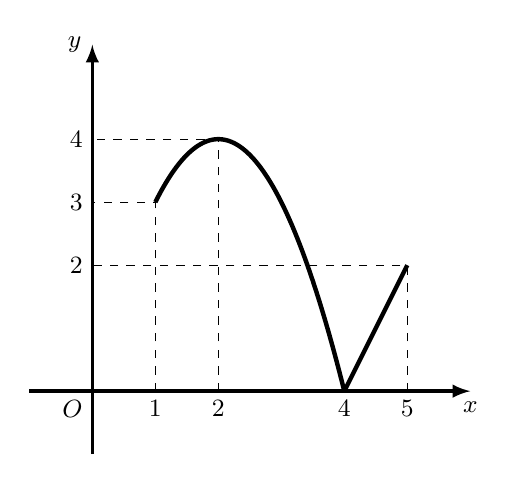
\begin{tikzpicture}[>=latex, scale=0.8]
    % 1. Hệ trục tọa độ Ox, Oy dày và rõ nét
    \draw[->, line width=1.2pt] (-1,0) -- (6,0) node[below] {\small $x$};
    \draw[->, line width=1.2pt] (0,-1) -- (0,5.5) node[left] {\small $y$};
    \node[below left] at (0,0) {\small $O$};
    
    % 2. Đồ thị hàm số từng nhánh
    % Nhánh 1: Parabol từ x = 1 (y = 3) đạt cực đại tại đỉnh x = 2 (y = 4) xuôi xuống x = 4 (y = 0)
    % Hàm phù hợp: y = -(x-2)^2 + 4
    \draw[ultra thick, samples=150, domain=1:4] plot (\x, {-(\x-2)*(\x-2) + 4});
    % Nhánh 2: Đoạn thẳng từ (4, 0) lên (5, 2)
    \draw[ultra thick] (4,0) -- (5,2);

    % 3. Đường nét đứt và điền số trục tọa độ
    % Tại x = 1, y = 3
    \draw[dashed] (1,0) -- (1,3) -- (0,3);
    \node[below] at (1,0) {\small $1$};
    \node[left] at (0,3) {\small $3$};
    
    % Tại x = 2, y = 4 (Đỉnh)
    \draw[dashed] (2,0) -- (2,4) -- (0,4);
    \node[below] at (2,0) {\small $2$};
    \node[left] at (0,4) {\small $4$};
    
    % Tại x = 4, y = 0
    \node[below] at (4,0) {\small $4$};
    
    % Tại x = 5, y = 2
    \draw[dashed] (5,0) -- (5,2) -- (0,2);
    \node[below] at (5,0) {\small $5$};
    \node[left] at (0,2) {\small $2$};

\end{tikzpicture}
\end{center}

Trên đoạn \([1; 5]\), hàm số đã cho đạt giá trị lớn nhất tại điểm}{
    \begin{tasks}(4)
        \task \( x = 4 \)
        \task \( x = 1 \)
        \task \( x = 2 \)
        \task \( x = 5 \)
    \end{tasks}
}

% --- CÂU 8 (tương ứng Câu 30 gốc: THPT Ngô Sĩ Liên) ---
\questionLinesManual{0}{8}{ Cho hàm số \( f(x) \) liên tục trên \([-1; 5]\) và có đồ thị trên đoạn \([-1; 5]\) như hình vẽ bên dưới. Tổng giá trị lớn nhất và giá trị nhỏ nhất của hàm số \( f(x) \) trên đoạn \([-1; 5]\) bằng

\begin{center}
\begin{tikzpicture}[>=latex, scale=0.8]
    % 1. Hệ trục tọa độ Ox, Oy
    \draw[->] (-2,0) -- (6,0) node[below] {\small $x$};
    \draw[->] (0,-3) -- (0,4) node[right] {\small $y$};
    \node[below left] at (0,0) {\small $0$};
    
    % 2. Đồ thị hàm số (vẽ bằng lệnh plot trơn tru qua các điểm cực trị)
    % Các điểm uốn và cực trị: (-1, -2), (0, 1) [Cực đại], (2, -2) [Cực tiểu], (4.25, 3) [Cực đại], (5, 1)
    \draw[thick,samples=150, domain=-1:5]
plot (\x, {-0.1588135590717*\x*\x*\x*\x + 1.2862146877635*\x*\x*\x - 2.3097740105484*\x*\x - 0.7548022573836*\x + 1});    % 3. Đường nét đứt và điền số trục tọa độ
    % Tại x = -1, y = -2
    \draw[dashed] (-1,0) -- (-1,-2) -- (0,-2);
    \node[above] at (-1,0) {\small $-1$};
    \node[below left] at (0,-2) {\small $-2$};
    
    % Tại x = 0, y = 1
    \node[above left] at (0,1) {\small $1$};
    
    % Tại x = 2, y = -2
    \draw[dashed] (2,0) -- (2,-2);
    \node[above] at (2,0) {\small $2$};
    
    % Tại đỉnh cực đại thứ hai (x ≈ 4.25, y = 3)
    \draw[dashed] (4.25,0) -- (4.25,3) -- (0,3);
    \node[left] at (0,3) {\small $3$};
    
    % Tại điểm cuối cùng x = 5, y = 1
    \draw[dashed] (5,0) -- (5,1) -- (0,1);
    \node[below] at (5,0) {\small $5$};

\end{tikzpicture}
\end{center}

}{
    \begin{tasks}(4)
        \task $4$
        \task $1$
        \task $2$
        \task $-1$
    \end{tasks}
}

% --- CÂU 9 (tương ứng Câu 32 gốc: THPT Hoằng Hóa 2) ---
\questionLinesManual{0}{9}{ Cho hàm số \( f(x) \) liên tục trên đoạn \([-2; 2]\) có đồ thị như hình vẽ. Gọi \( M \) và \( m \) lần lượt là giá trị lớn nhất và nhỏ nhất của hàm số trên đoạn \([-2; 2]\). Khi đó, tổng \( M + m \) bằng

\begin{center}
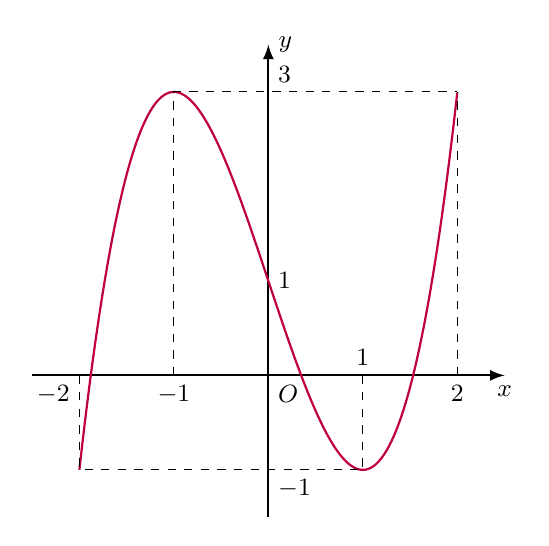
\begin{tikzpicture}[>=latex, scale=1.2]
    % 1. Hệ trục tọa độ Ox, Oy màu đen
    \draw[->, black, thick] (-2.5, 0) -- (2.5, 0) node[below] {\small $x$};
    \draw[->, black, thick] (0, -1.5) -- (0, 3.5) node[right] {\small $y$};
    \node[below right] at (0,0) {\small $O$};
    
    % 2. Đồ thị hàm số bậc ba màu tím (Purple)
    % Hàm số mẫu chính xác đi qua các điểm: 
    % Cực đại (-1, 3), Cực tiểu (1, -1), Cắt Oy tại (0, 1), f(2) = 3, f(-2) = -1
    % Công thức: y = x^3 - 3x + 1
    \draw[purple, thick, samples=150, domain=-2:2] plot (\x, {\x*\x*\x - 3*\x + 1});

    % 3. Các đường nét đứt và nhãn tọa độ màu đen
    % Tại x = -2, y = -1
    \draw[dashed, black] (-2,0) -- (-2,-1) -- (1,-1);
    \node[below left] at (-2,0) {\small $-2$};
    
    % Tại x = -1, y = 3 (Cực đại)
    \draw[dashed, black] (-1,0) -- (-1,3) -- (2,3);
    \node[below] at (-1,0) {\small $-1$};
    
    % Tại giao điểm Oy (x = 0, y = 1)
    \node[right] at (0,1) {\small $1$};
    
    % Tại x = 1, y = -1 (Cực tiểu)
    \draw[dashed, black] (1,0) -- (1,-1);
    \node[above] at (1,0) {\small $1$};
    \node[below right] at (0,-1) {\small $-1$};
    
    % Tại x = 2, y = 3
    \draw[dashed, black] (2,0) -- (2,3);
    \node[below] at (2,0) {\small $2$};
    \node[above right] at (0,3) {\small $3$};

\end{tikzpicture}
\end{center}

}{
    \begin{tasks}(4)
        \task $-6$
        \task $-2$
        \task $-5$
        \task $2$
    \end{tasks}
}

% --- CÂU 10 (tương ứng Câu 34 gốc: THPT Tư Nghĩa 1) ---
\questionLinesManual{0}{10}{Cho hàm số \( y = f(x) \) có đồ thị trên đoạn \([-3; 5]\) như hình vẽ. Gọi \( M, m \) lần lượt là giá trị lớn nhất và giá trị nhỏ nhất của hàm số đã cho trên đoạn \([-3; 5]\). Tính \( 2M - m \).

\begin{center}
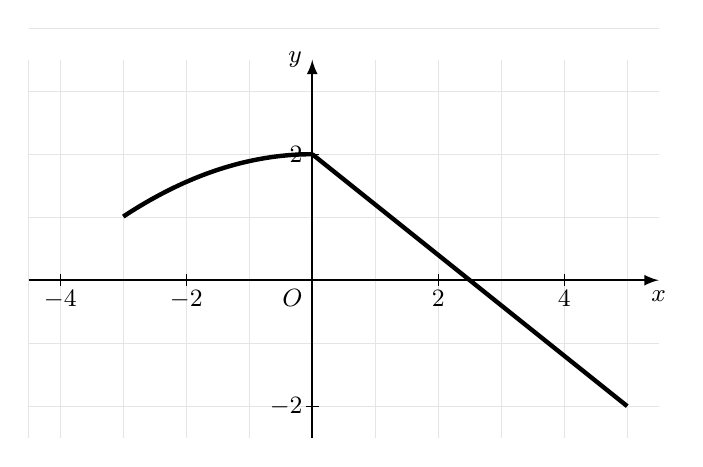
\begin{tikzpicture}[>=latex, scale=0.8]
    % 1. Vẽ lưới ô vuông (grid) màu xám nhạt phía sau đồ thị
    \draw[color=gray!20, thin, step=1] (-4.5,-2.5) -- (-4.5,3.5) grid (5.5,3.5);
    \draw[color=gray!20, thin] (-4.5,-2.5) grid (5.5,3.5);

    % 2. Hệ trục tọa độ Ox, Oy màu đen
    \draw[->, black, thick] (-4.5, 0) -- (5.5, 0) node[below] {\small $x$};
    \draw[->, black, thick] (0, -2.5) -- (0, 3.5) node[left] {\small $y$};
    \node[below left] at (0,0) {\small $O$};
    
    % Các vạch chia và số trên trục hoành Ox
    \foreach \x in {-4, -2, 2, 4} {
        \draw[black] (\x, 0.1) -- (\x, -0.1);
        \node[below] at (\x, 0) {\small $\x$};
    }
    
    % Các vạch chia và số trên trục tung Oy
    \draw[black] (0.1, 2) -- (-0.1, 2);
    \node[left] at (0, 2) {\small $2$};
    \draw[black] (0.1, -2) -- (-0.1, -2);
    \node[left] at (0, -2) {\small $-2$};

    % 3. Đồ thị hàm số màu đen (black)
    % Nhánh trái: từ x = -3 đến x = 0
    \draw[black, ultra thick, samples=100, domain=-3:0] plot (\x, {2 - 0.11*\x*\x});
    
    % Nhánh phải: đoạn thẳng tuyến tính từ x = 0 đến x = 5
    \draw[black, ultra thick] (0,2) -- (5,-2);

\end{tikzpicture}
\end{center}

}{
    \begin{tasks}(4)
        \task $5$
        \task $8$
        \task $2$
        \task $6$
    \end{tasks}
}

% --- CÂU 11 (tương ứng Câu 37 gốc: Cụm Chuyên Môn Đăk Lak) ---
\questionLinesManual{0}{11}{ Cho hàm số \( y = f(x) \), có đồ thị trên đoạn \([-2; 2]\) như hình vẽ.

\begin{center}
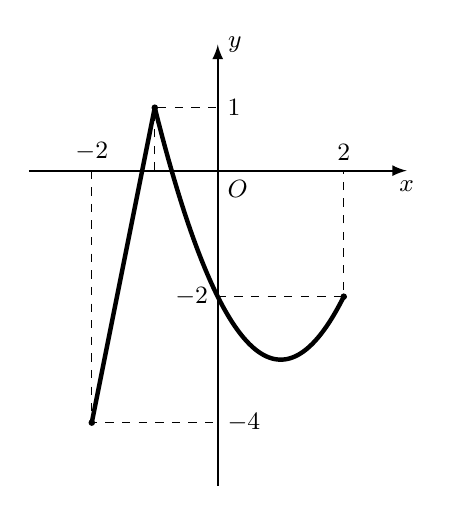
\begin{tikzpicture}[>=latex, scale=0.8]
    % 1. Hệ trục tọa độ Ox, Oy màu đen
    \draw[->, black, thick] (-3,0) -- (3,0) node[below] {\small $x$};
    \draw[->, black, thick] (0,-5) -- (0,2) node[right] {\small $y$};
    \node[below right] at (0,0) {\small $O$};
    
    % 2. Đồ thị hàm số màu đen chia làm 2 nhánh nối nhau tại điểm x = -1, y = 1
    % Nhánh trái: đoạn thẳng từ (-2, -4) lên cực đại tại (-1, 1)
    \draw[black, ultra thick] (-2,-4) -- (-1,1);
    \filldraw[black] (-2,-4) circle (1.2pt);
    \filldraw[black] (-1,1) circle (1.2pt);

    % Nhánh phải: đường cong từ (-1, 1) qua (0, -2) xuống cực tiểu rồi lên (2, -2)
    % Hàm mẫu parabol phù hợp cho nhánh này: y = x^2 - 2x - 2 trên miền [-1; 2]
    % Tại x = -1 -> y = 1
    % Tại x = 0  -> y = -2
    % Tại x = 1  -> y = -3 (Đỉnh cực tiểu)
    % Tại x = 2  -> y = -2
    \draw[black, ultra thick, samples=150, domain=-1:2] plot (\x, {\x*\x - 2*\x - 2});
    \filldraw[black] (2,-2) circle (1.2pt);

    % 3. Các đường nét đứt và nhãn tọa độ màu đen
    % Tại x = -2, y = -4
    \draw[dashed, black] (-2,0) -- (-2,-4) -- (0,-4);
    \node[above] at (-2,0) {\small $-2$};
    \node[right] at (0,-4) {\small $-4$};
    
    % Tại cực đại x = -1, y = 1
    \draw[dashed, black] (-1,0) -- (-1,1) -- (0,1);
    \node[right] at (0,1) {\small $1$};
    
    % Tại điểm giao Oy (x = 0, y = -2) và điểm mút (2, -2)
    \draw[dashed, black] (0,-2) -- (2,-2) -- (2,0);
    \node[left] at (0,-2) {\small $-2$};
    \node[above] at (2,0) {\small $2$};

\end{tikzpicture}
\end{center}

Gọi giá trị lớn nhất và giá trị nhỏ nhất của hàm số \( f(x) \) trên \([-2; 2]\) lần lượt là \( M \) và \( m \). Khi đó \( M - m \) bằng:

}{
    \begin{tasks}(4)
        \task $5$
        \task $3$
        \task $-4$
        \task $0$
    \end{tasks}
}

% --- CÂU 12 (tương ứng Câu 38 gốc: Cụm Chuyên Môn Đăk Lak) ---
\questionLinesManual{0}{12}{Cho hàm số \( y = f(x) \) có đồ thị như hình vẽ. Giá trị lớn nhất của hàm số \( y = f(x) \) trên đoạn \([-2; 0]\) bằng:

\begin{center}
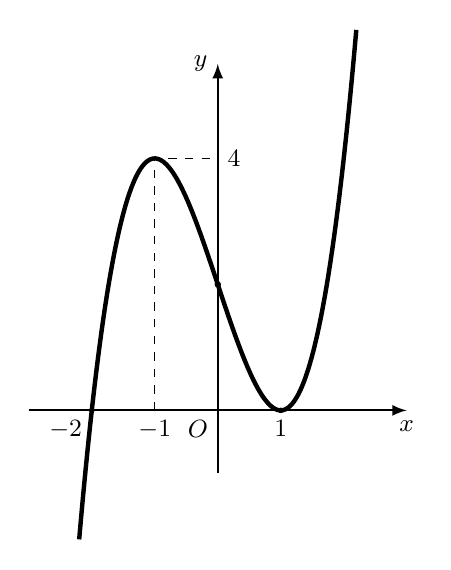
\begin{tikzpicture}[>=latex, scale=0.8]
    % 1. Hệ trục tọa độ Ox, Oy màu đen
    \draw[->, black, thick] (-3,0) -- (3,0) node[below] {\small $x$};
    \draw[->, black, thick] (0,-1) -- (0,5.5) node[left] {\small $y$};
    \node[below left] at (0,0) {\small $O$};
    
    % 2. Đồ thị hàm số bậc ba màu đen
    % Hàm mẫu phù hợp: y = x^3 - 3x + 2
    % Tại x = -2 -> y = 0 (Giao điểm hoành độ bên trái)
    % Tại x = -1 -> y = 4 (Cực đại)
    % Tại x = 0  -> y = 2 (Giao điểm Oy)
    % Tại x = 1  -> y = 0 (Cực tiểu tiếp xúc Ox)
    \draw[black, ultra thick, samples=150, domain=-2.2:2.2] plot (\x, {\x*\x*\x - 3*\x + 2});
    
    % Điểm chấm đen tại giao điểm trục Oy (0,2)
    \filldraw[black] (0,2) circle (1.2pt);

    % 3. Các đường nét đứt và nhãn tọa độ màu đen
    % Tại giao điểm hoành độ phía âm
    \node[below left] at (-2,0) {\small $-2$};
    \filldraw[black] (-2,0) circle (1pt);
    
    % Tại cực đại x = -1, y = 4
    \draw[dashed, black] (-1,0) -- (-1,4) -- (0,4);
    \node[below] at (-1,0) {\small $-1$};
    \node[right] at (0,4) {\small $4$};
    
    % Tại cực tiểu x = 1, y = 0
    \node[below] at (1,0) {\small $1$};
    \filldraw[black] (1,0) circle (1pt);

\end{tikzpicture}
\end{center}

}{
    \begin{tasks}(4)
        \task $1$
        \task $4$
        \task $-2$
        \task $-1$
    \end{tasks}
}

% --- CÂU 13 (tương ứng Câu 1 gốc: Đề Tham Khảo 2019) ---
\questionLinesManual{0}{13}{ Cho hàm số \( y = f(x) \) liên tục trên đoạn \([-1; 3]\) và có đồ thị như hình vẽ bên. Gọi \( M \) và \( m \) lần lượt là giá trị lớn nhất và nhỏ nhất của hàm số đã cho trên đoạn \([-1; 3]\). Giá trị của \( M - m \) bằng

\begin{center}
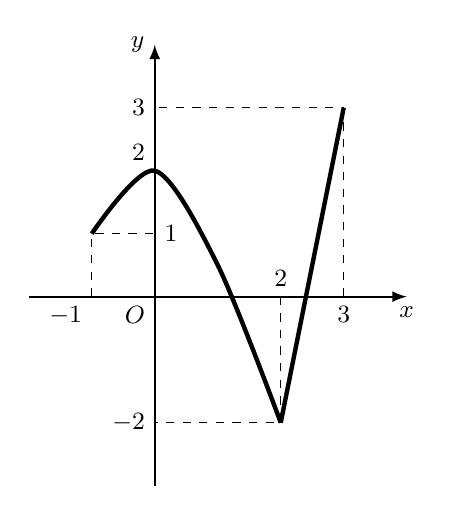
\begin{tikzpicture}[>=latex, scale=0.8]
    % 1. Hệ trục tọa độ Ox, Oy màu đen
    \draw[->, black, thick] (-2,0) -- (4,0) node[below] {\small $x$};
    \draw[->, black, thick] (0,-3) -- (0,4) node[left] {\small $y$};
    \node[below left] at (0,0) {\small $O$};
    
    % 2. Đồ thị hàm số màu đen chia làm 2 nhánh chính nối nhau tại cực tiểu (2, -2)
    % Nhánh trái: parabol/đường cong từ (-1, 1) đạt cực đại tại (0, 2) rồi đi xuống (2, -2)
    % Hàm phù hợp: y = -x^2 + 2 trên miền [-1; 0], sau đó chuyển tiếp mượt sang x = 2
    % Để đơn giản và chính xác theo hình dáng, sử dụng plot qua các tọa độ:
    \draw[black, ultra thick, samples=100] plot[smooth, domain=-1:2] coordinates {(-1,1) (0,2) (1,0.5) (2,-2)};
    
    % Nhánh phải: đoạn thẳng từ cực tiểu (2, -2) lên điểm mút (3, 3)
    \draw[black, ultra thick] (2,-2) -- (3,3);

    % 3. Các đường nét đứt và nhãn tọa độ màu đen
    % Tại điểm đầu mút x = -1, y = 1
    \draw[dashed, black] (-1,0) -- (-1,1) -- (0,1);
    \node[below left] at (-1,0) {\small $-1$};
    \node[right] at (0,1) {\small $1$};
    
    % Tại điểm cực đại y = 2 trên trục Oy
    \node[above left] at (0,2) {\small $2$};
    
    % Tại cực tiểu x = 2, y = -2
    \draw[dashed, black] (2,0) -- (2,-2) -- (0,-2);
    \node[above] at (2,0) {\small $2$};
    \node[left] at (0,-2) {\small $-2$};
    
    % Tại điểm đầu mút x = 3, y = 3
    \draw[dashed, black] (3,0) -- (3,3) -- (0,3);
    \node[below] at (3,0) {\small $3$};
    \node[left] at (0,3) {\small $3$};

\end{tikzpicture}
\end{center}

}{
    \begin{tasks}(4)
        \task $1$
        \task $4$
        \task $5$
        \task $0$
    \end{tasks}
}

% --- CÂU 14 (tương ứng Câu 5 gốc: Chuyên Lương Thế Vinh Đồng Nai) ---
\questionLinesManual{0}{14}{Cho hàm số \( y = f(x) \) xác định và liên tục trên \( \mathbb{R} \) có đồ thị như hình vẽ bên. Tìm giá trị nhỏ nhất \( m \) và giá trị lớn nhất \( M \) của hàm số \( y = f(x) \) trên đoạn \([-2; 2]\).

\begin{center}
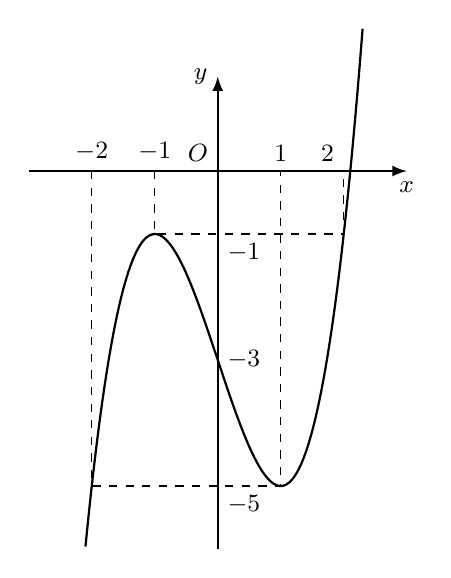
\begin{tikzpicture}[>=latex, scale=0.8]
    % 1. Hệ trục tọa độ Ox, Oy màu đen
    \draw[->, black, thick] (-3,0) -- (3,0) node[below] {\small $x$};
    \draw[->, black, thick] (0,-6) -- (0,1.5) node[left] {\small $y$};
    \node[above left] at (0,0) {\small $O$};
    
    % 2. Đồ thị hàm số bậc ba màu đen
    % Hàm mẫu phù hợp: y = x^3 - 3x - 3
    % Tại x = -2 -> y = -5
    % Tại x = -1 -> y = -1 (Cực đại)
    % Tại x = 0  -> y = -3 (Giao điểm Oy)
    % Tại x = 1  -> y = -5 (Cực tiểu)
    % Tại x = 2  -> y = -1
    \draw[thick, samples=150, domain=-2.1:2.3] plot (\x, {\x*\x*\x - 3*\x - 3});

    % 3. Các đường nét đứt và nhãn tọa độ màu đen
    % Các mốc trên trục hoành
    \node[above] at (-2,0) {\small $-2$};
    \node[above] at (-1,0) {\small $-1$};
    \node[above] at (1,0) {\small $1$};
    \node[above left] at (2,0) {\small $2$};

    % Các mốc trên trục tung
    \node[below right] at (0,-1) {\small $-1$};
    \node[right] at (0,-3) {\small $-3$};
    \node[below right] at (0,-5) {\small $-5$};

    % Đường nét đứt tại cực đại y = -1 (nối từ x = -1 sang x = 2)
    \draw[dashed, black] (-1,0) -- (-1,-1) -- (2,-1) -- (2,0);
    
    % Đường nét đứt tại cực tiểu y = -5 (nối từ x = -2 sang x = 1)
    \draw[dashed, black] (-2,0) -- (-2,-5) -- (1,-5) -- (1,0);

\end{tikzpicture}
\end{center}

}{
    \begin{tasks}(4)
        \task \( m = -5; M = -1 \)
        \task \( m = -2; M = 2 \)
        \task \( m = -1; M = 0 \)
        \task \( m = -5; M = 0 \)
    \end{tasks}
}

% --- CÂU 15 (tương ứng Câu 9 gốc: VTED 2019) ---
\questionLinesManual{0}{15}{ Cho hàm số \( f(x) \) liên tục trên \([-1; 5]\) và có đồ thị trên đoạn \([-1; 5]\) như hình vẽ bên dưới. Tổng giá trị lớn nhất và giá trị nhỏ nhất của hàm số \( f(x) \) trên đoạn \([-1; 5]\) bằng

\begin{center}
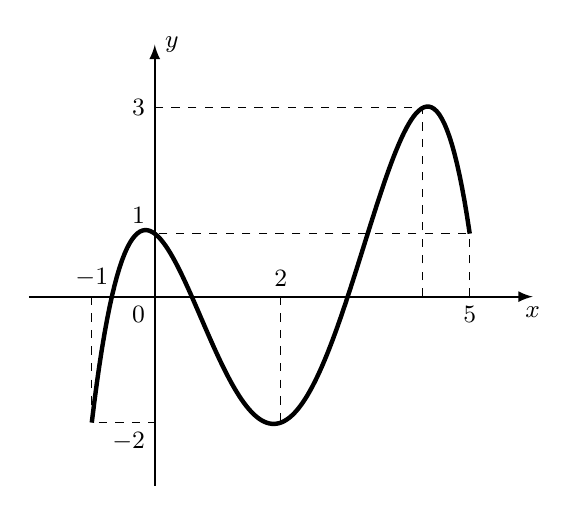
\begin{tikzpicture}[>=latex, scale=0.8]
    % 1. Hệ trục tọa độ Ox, Oy màu đen
    \draw[->, black, thick] (-2,0) -- (6,0) node[below] {\small $x$};
    \draw[->, black, thick] (0,-3) -- (0,4) node[right] {\small $y$};
    \node[below left] at (0,0) {\small $0$};
    
    % 2. Đồ thị hàm số màu đen
    \draw[black, ultra thick, samples=150, domain=-1:5] 
plot (\x, {-0.1588135590717*\x*\x*\x*\x + 1.2862146877635*\x*\x*\x - 2.3097740105484*\x*\x - 0.7548022573836*\x + 1});
    % 3. Các đường nét đứt và nhãn tọa độ màu đen
    % Tại x = -1, y = -2
    \draw[dashed, black] (-1,0) -- (-1,-2) -- (0,-2);
    \node[above] at (-1,0) {\small $-1$};
    \node[below left] at (0,-2) {\small $-2$};
    
    % Tại x = 0, y = 1
    \node[above left] at (0,1) {\small $1$};
    
    % Tại x = 2, y = -2
    \draw[dashed, black] (2,0) -- (2,-2);
    \node[above] at (2,0) {\small $2$};
    
    % Tại đỉnh cực đại thứ hai (x ≈ 4.25, y = 3)
    \draw[dashed, black] (4.25,0) -- (4.25,3) -- (0,3);
    \node[left] at (0,3) {\small $3$};
    
    % Tại điểm cuối cùng x = 5, y = 1
    \draw[dashed, black] (5,0) -- (5,1) -- (0,1);
    \node[below] at (5,0) {\small $5$};

\end{tikzpicture}
\end{center}

}{
    \begin{tasks}(4)
        \task $-1$
        \task $4$
        \task $1$
        \task $2$
    \end{tasks}
}

% --- CÂU 16 (tương ứng Câu 10 gốc: THPT Yên Mỹ Hưng Yên) ---
\questionLinesManual{0}{16}{ Cho hàm số \( y = f(x) \) xác định, liên tục trên \([-1, \dfrac{5}{2}]\) và có đồ thị là đường cong như hình vẽ.

\begin{center}
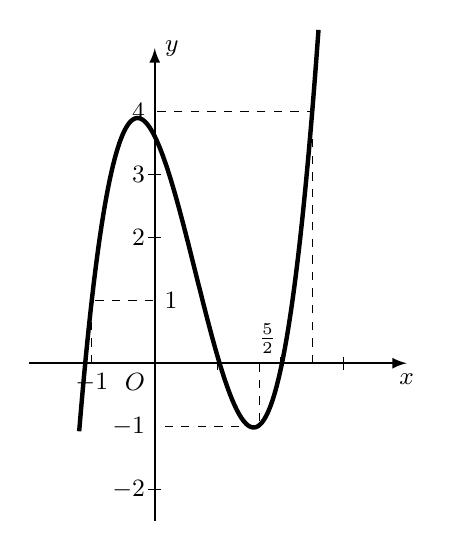
\begin{tikzpicture}[>=latex, scale=0.8]
    % 1. Hệ trục tọa độ Ox, Oy màu đen và các vạch chia nhỏ (ticks)
    \draw[->, black, thick] (-2,0) -- (4,0) node[below] {\small $x$};
    \draw[->, black, thick] (0,-2.5) -- (0,5) node[right] {\small $y$};
    \node[below left] at (0,0) {\small $O$};
    
    % Các vạch chia nhỏ trên trục Ox
    \foreach \x in {1, 2, 3} {
        \draw[black] (\x, 0.1) -- (\x, -0.1);
    }
    % Các vạch chia nhỏ trên trục Oy
    \foreach \y in {2, 3} {
        \draw[black] (0.1, \y) -- (-0.1, \y);
        \node[left] at (0,\y) {\small $\y$};
    }

    % 2. Đồ thị hàm số bậc ba màu đen
    % Hàm số mẫu phù hợp: y = 2x^3 - 5x^2 + 3.5 (hoặc vẽ mượt qua các điểm cực trị bằng coordinates)
    \draw[black, ultra thick, samples=150, domain=-1.2:2.6] 
  plot (\x, {1.5695238095238*\x*\x*\x - 3.0514285714286*\x*\x - 2.0209523809524*\x + 3.6});
    % 3. Các đường nét đứt và nhãn tọa độ màu đen
    % Tại điểm x = -1, y = 1
    \draw[dashed, black] (-1,0) -- (-1,1) -- (0,1);
    \node[below] at (-1,0) {\small $-1$};
    \node[right] at (0,1) {\small $1$};
    
    % Tại điểm cực tiểu (x = 5/2, y = -1) - Lưu ý ký hiệu 5/2 nằm ở vị trí hoành độ cực tiểu trong hình
    \draw[dashed, black] (1.66,0) -- (1.66,-1) -- (0,-1);
    \node[above right] at (1.5,0) {\small $\frac{5}{2}$};
    \node[left] at (0,-1) {\small $-1$};
    
    % Mốc y = -2 trên trục Oy
    \draw[black] (0.1, -2) -- (-0.1, -2);
    \node[left] at (0,-2) {\small $-2$};

    % Tại điểm mút phía trên x = 2.5, y = 4
    \draw[dashed, black] (2.5,0) -- (2.5,4) -- (0,4);
    \node[left] at (0,4) {\small $4$};

\end{tikzpicture}
\end{center}

Giá trị lớn nhất \( M \) và giá trị nhỏ nhất \( m \) của hàm số \( f(x) \) trên \([-1, \dfrac{5}{2}]\) là:

}{
    \begin{tasks}(4)
        \task \( M = 4, m = 1 \)
        \task \( M = 4, m = -1 \)
        \task \( M = \dfrac{7}{2}, m = -1 \)
        \task \( M = \dfrac{7}{2}, m = 1 \)
    \end{tasks}
}

% --- CÂU 17 (tương ứng Câu 12 gốc: Sở Bắc Giang 2019) ---
\questionLinesManual{0}{17}{ Cho hàm số \( y = f(x) \) liên tục trên đoạn \([-1; 3]\) và có đồ thị như hình vẽ bên. Gọi \( M, m \) lần lượt là giá trị lớn nhất và giá trị nhỏ nhất của hàm số đã cho trên đoạn \([-1; 3]\). Giá trị của \( M + m \) là

\begin{center}
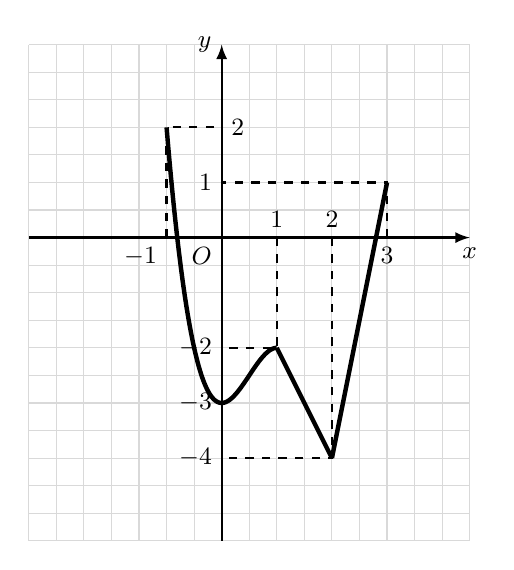
\begin{tikzpicture}[>=latex, scale=0.7]
    % 1. Vẽ lưới ô vuông (grid) màu xám nhạt phía sau đồ thị
    \draw[color=gray!30, thin, step=0.5] (-3.5,-5.5) grid (4.5,3.5);

    % 2. Hệ trục tọa độ Ox, Oy màu đen
    \draw[->, black, thick] (-3.5, 0) -- (4.5, 0) node[below] {\small $x$};
    \draw[->, black, thick] (0, -5.5) -- (0, 3.5) node[left] {\small $y$};
    \node[below left] at (0,0) {\small $O$};

    % 3. Đồ thị hàm số màu đen (black, ultra thick) từng nhánh
    % Nhánh 1: Đường cong mượt từ x = -1 (y = 2) qua (0, -3) đến cực đại (1, -2)
    \draw[black, ultra thick, samples=100, domain=-1:1] plot (\x, {-2*\x*\x*\x + 3*\x*\x - 3});
    
    % Nhánh 2: Đoạn thẳng từ (1, -2) xuống (2, -4)
    \draw[black, ultra thick] (1,-2) -- (2,-4);
    
    % Nhánh 3: Đoạn thẳng từ (2, -4) lên điểm mút (3, 1)
    \draw[black, ultra thick] (2,-4) -- (3,1);

    % 4. Các đường nét đứt và nhãn tọa độ màu đen
    % Tại x = -1, y = 2
    \draw[dashed, black, thick] (-1,0) -- (-1,2) -- (0,2);
    \node[below left] at (-1,0) {\small $-1$};
    \node[right] at (0,2) {\small $2$};
    
    % Mốc y = -3 và y = 1 trên Oy
    \node[left] at (0,-3) {\small $-3$};
    \node[left] at (0,1) {\small $1$};
    
    % Tại x = 1, y = -2
    \draw[dashed, black, thick] (1,0) -- (1,-2) -- (0,-2);
    \node[above] at (1,0) {\small $1$};
    \node[left] at (0,-2) {\small $-2$};
    
    % Tại x = 2, y = -4
    \draw[dashed, black, thick] (2,0) -- (2,-4) -- (0,-4);
    \node[above] at (2,0) {\small $2$};
    \node[left] at (0,-4) {\small $-4$};
    
    % Tại x = 3, y = 1
    \draw[dashed, black, thick] (3,0) -- (3,1) -- (0,1);
    \node[below] at (3,0) {\small $3$};

\end{tikzpicture}
\end{center}

}{
    \begin{tasks}(4)
        \task $2$
        \task $-6$
        \task $-5$
        \task $-2$
    \end{tasks}
}

% --- CÂU 18 (tương ứng Câu 14 gốc) ---
\questionLinesManual{0}{18}{Cho hàm số \( f(x) \) liên tục trên đoạn \([0;3]\) và có đồ thị như hình vẽ bên. Gọi \( M \) và \( m \) lần lượt là giá trị lớn nhất và nhỏ nhất của hàm số đã cho trên \([0;3]\). Giá trị của \( M + m \) bằng?

\begin{center}
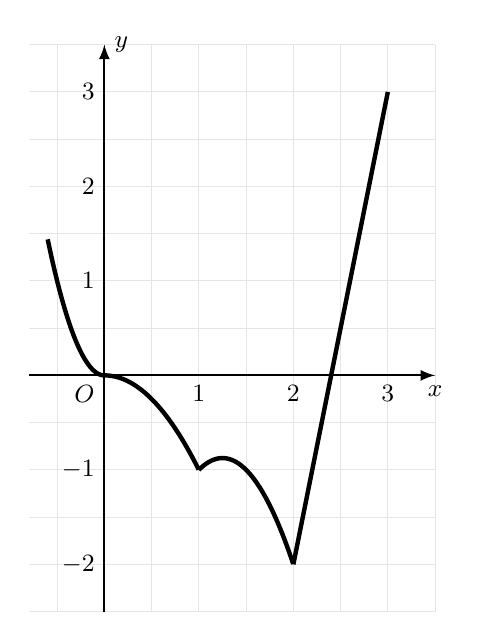
\begin{tikzpicture}[>=latex, scale=1.2]
    % 1. Vẽ lưới ô vuông (grid) phía sau đồ thị
    \draw[color=gray!20, thin, step=0.5] (-0.8,-2.5) grid (3.5,3.5);

    % 2. Hệ trục tọa độ Ox, Oy màu đen
    \draw[->, black, thick] (-0.8, 0) -- (3.5, 0) node[below] {\small $x$};
    \draw[->, black, thick] (0, -2.5) -- (0, 3.5) node[right] {\small $y$};
    \node[below left] at (0,0) {\small $O$};
    
    % Các số chỉ mục trên trục hoành Ox
    \node[below] at (1, 0) {\small $1$};
    \node[below] at (2, 0) {\small $2$};
    \node[below] at (3, 0) {\small $3$};
    
    % Các số chỉ mục trên trục tung Oy
    \node[left] at (0, 1) {\small $1$};
    \node[left] at (0, 2) {\small $2$};
    \node[left] at (0, 3) {\small $3$};
    \node[left] at (0, -1) {\small $-1$};
    \node[left] at (0, -2) {\small $-2$};

    % 3. Đồ thị hàm số màu đen chia thành các nhánh
    % Nhánh 1: Đường cong phía bên trái trục Oy đi xuống gốc tọa độ O(0,0)
    \draw[black, ultra thick, samples=100, domain=-0.6:0] plot (\x, {4*\x*\x});

    % Nhánh 2: Đường cong từ O(0,0) xuống góc nhọn tại (1, -1)
    \draw[black, ultra thick, samples=100, domain=0:1] plot (\x, {-\x*\x});

    % Nhánh 3: Đường cong từ (1, -1) lên cực đại địa phương tại x=1.35 rồi xuống cực tiểu nhọn tại (2, -2)
    % Hàm mẫu parabol úp phù hợp: y = -4*(x-1.35)^2 - 0.5
    \draw[black, ultra thick, samples=100, domain=1:2] plot (\x, {-2*\x^2 + 5*\x - 4});

    % Nhánh 4: Đường cong từ cực tiểu (2, -2) đi lên qua các ô lưới đến x=3.2
    \draw[black, ultra thick, samples=100] (2,-2) -- (3,3);
\end{tikzpicture}
\end{center}

}{
    \begin{tasks}(4)
        \task $5$
        \task $3$
        \task $2$
        \task $1$
    \end{tasks}
}

% --- CÂU 19 (tương ứng Câu 15 gốc: Chuyên Lê Quý Đôn Điện Biên) ---
\questionLinesManual{0}{19}{ Cho hàm số \( y = f(x) \) liên tục trên đoạn \([-2;6]\) và có đồ thị như hình vẽ bên dưới.

\begin{center}
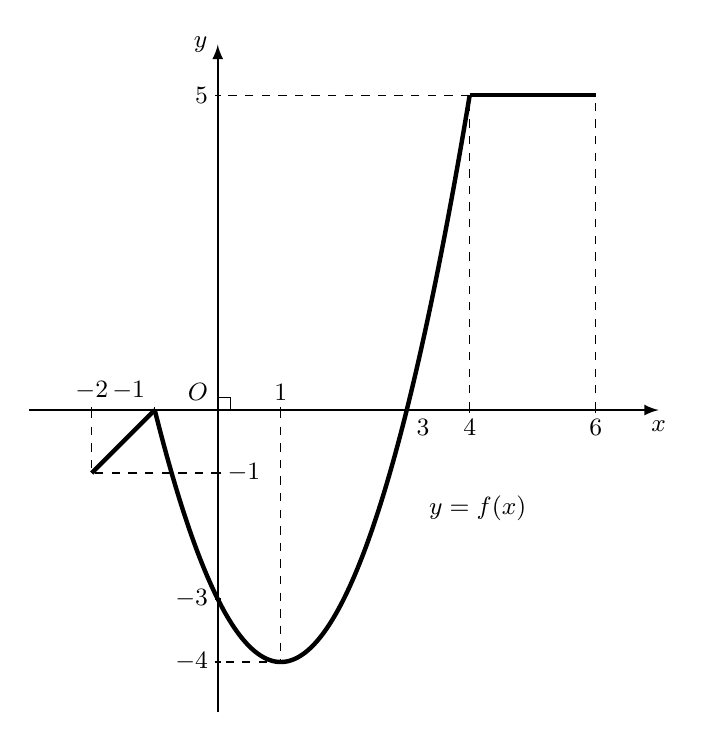
\begin{tikzpicture}[>=latex, scale=0.8]
    % 1. Hệ trục tọa độ Ox, Oy màu đen và ký hiệu vuông góc
    \draw[->, black, thick] (-3,0) -- (7,0) node[below] {\small $x$};
    \draw[->, black, thick] (0,-4.8) -- (0,5.8) node[left] {\small $y$};
    \node[above left] at (0,0) {\small $O$};
    \draw[black] (0,0.2) -- (0.2,0.2) -- (0.2,0); % Ký hiệu vuông góc tại gốc O

    % Các vạch nhỏ chia tọa độ trên trục Ox và Oy
    \foreach \x in {-2, -1, 1, 3, 4, 6} \draw[black] (\x, 0.05) -- (\x, -0.05);
    \foreach \y in {-4, -3, -1, 5} \draw[black] (0.05, \y) -- (-0.05, \y);

    % 2. Đồ thị hàm số màu đen gồm các nhánh liền mạch
    % Nhánh 1: Đoạn thẳng từ (-2, -1) lên (-1, 0)
    \draw[black, ultra thick] (-2,-1) -- (-1,0);
    
    % Nhánh 2: Parabol từ (-1, 0) qua (0, -3), đạt cực tiểu tại (1, -4) rồi đi lên cắt Ox tại x = 3 đến điểm (4, 5)
    \draw[black, ultra thick, samples=150, domain=-1:4] plot (\x, {\x*\x - 2*\x - 3});
    
    % Nhánh 3: Đoạn thẳng nằm ngang từ (4, 5) đến điểm mút (6, 5)
    \draw[black, ultra thick] (4,5) -- (6,5);
    
    % Nhãn tên đồ thị y = f(x)
    \node[below right] at (3.2,-1.2) {\small $y = f(x)$};

    % 3. Các đường nét đứt và nhãn tọa độ màu đen
    % Tại mốc x = -2, y = -1
    \draw[dashed, black] (-2,0) -- (-2,-1) -- (0,-1);
    \node[above] at (-2,0) {\small $-2$};
    \node[above left] at (-1,0) {\small $-1$};
    \node[right] at (0,-1) {\small $-1$};
    
    % Tại vị trí cắt trục tung Oy tại y = -3
    \node[left] at (0,-3) {\small $-3$};
    
    % Tại cực tiểu x = 1, y = -4
    \draw[dashed, black] (1,0) -- (1,-4) -- (0,-4);
    \node[above] at (1,0) {\small $1$};
    \node[left] at (0,-4) {\small $-4$};
    
    % Tại vị trí cắt trục hoành x = 3
    \node[below right] at (3,0) {\small $3$};
    
    % Tại mốc x = 4, y = 5
    \draw[dashed, black] (4,0) -- (4,5) -- (0,5);
    \node[below] at (4,0) {\small $4$};
    \node[left] at (0,5) {\small $5$};
    
    % Tại điểm cuối cùng x = 6, y = 5
    \draw[dashed, black] (6,0) -- (6,5);
    \node[below] at (6,0) {\small $6$};

\end{tikzpicture}
\end{center}

Gọi \( M \) và \( m \) lần lượt là giá trị lớn nhất và nhỏ nhất của hàm số đã cho trên đoạn \([-2;6]\). Giá trị của \( M - m \) bằng}{
    \begin{tasks}(4)
        \task $9$
        \task $-8$
        \task $-9$
        \task $8$
    \end{tasks}
}

% --- CÂU 20 (tương ứng Câu 16 gốc: VTED 2019) ---
\questionLinesManual{0}{20}{Cho hàm số \( y = f(x) \) liên tục và có đồ thị trên đoạn \([-2; 4]\) như hình vẽ bên. Tổng giá trị lớn nhất và nhỏ nhất của hàm số \( y = f(x) \) trên đoạn \([-2; 4]\) bằng

\begin{center}
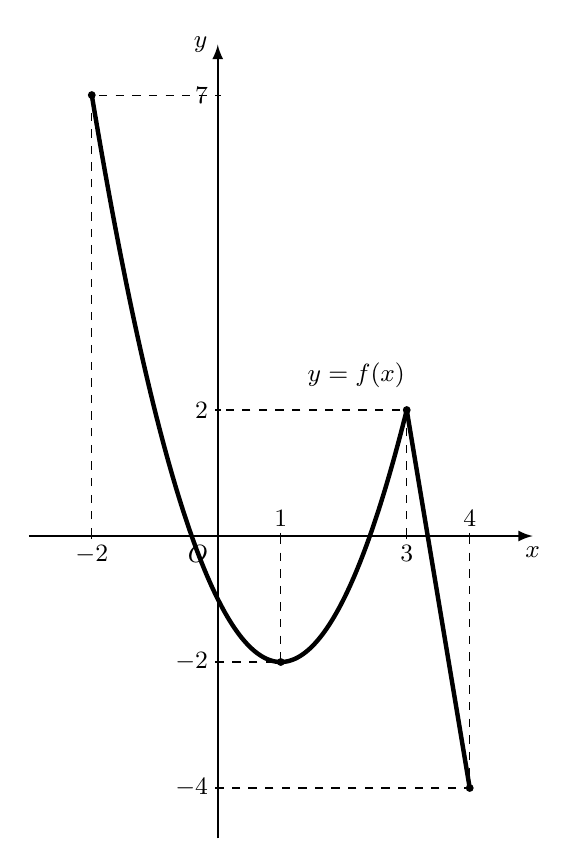
\begin{tikzpicture}[>=latex, scale=0.8]
    % 1. Hệ trục tọa độ Ox, Oy màu đen
    \draw[->, black, thick] (-3,0) -- (5,0) node[below] {\small $x$};
    \draw[->, black, thick] (0,-4.8) -- (0,7.8) node[left] {\small $y$};
    \node[below left] at (0,0) {\small $O$};

    % Các vạch nhỏ chia tọa độ trên trục Ox và Oy
    \foreach \x in {-2, 1, 3, 4} \draw[black] (\x, 0.05) -- (\x, -0.05);
    \foreach \y in {-4, -2, 2, 7} \draw[black] (0.05, \y) -- (-0.05, \y);

    % 2. Đồ thị hàm số màu đen gồm các nhánh liền mạch
    % Nhánh 1: Parabol/đường cong từ (-2, 7) đi xuống đạt cực tiểu tại (1, -2) rồi đi lên cực đại nhọn tại (3, 2)
    % Hàm mẫu phù hợp cho cung này: y = (x-1)^2 - 2 trên đoạn [-2, 3]
    \draw[black, ultra thick, samples=150, domain=-2:3] plot (\x, {(\x-1)*(\x-1) - 2});
    
    % Nhánh 2: Đoạn thẳng dốc xuống từ cực đại nhọn (3, 2) đến điểm mút (4, -4)
    \draw[black, ultra thick] (3,2) -- (4,-4);

    % Vẽ các điểm mút tròn tại các vị trí giới hạn (giữ màu đen đồng bộ)
    \filldraw[black] (-2,7) circle (1.5pt);
    \filldraw[black] (1,-2) circle (1.5pt);
    \filldraw[black] (3,2) circle (1.5pt);
    \filldraw[black] (4,-4) circle (1.5pt);

    % Tên đồ thị y = f(x)
    \node[above] at (2.2,2.2) {\small $y = f(x)$};

    % 3. Các đường nét đứt và nhãn tọa độ màu đen
    % Tại mốc x = -2, y = 7
    \draw[dashed, black] (-2,0) -- (-2,7) -- (0,7);
    \node[below] at (-2,0) {\small $-2$};
    \node[left] at (0,7) {\small $7$};
    
    % Tại mốc cực tiểu x = 1, y = -2
    \draw[dashed, black] (1,0) -- (1,-2) -- (0,-2);
    \node[above] at (1,0) {\small $1$};
    \node[left] at (0,-2) {\small $-2$};
    
    % Tại mốc cực đại nhọn x = 3, y = 2
    \draw[dashed, black] (3,0) -- (3,2) -- (0,2);
    \node[below] at (3,0) {\small $3$};
    \node[left] at (0,2) {\small $2$};
    
    % Tại mốc điểm mút cuối x = 4, y = -4
    \draw[dashed, black] (4,0) -- (4,-4) -- (0,-4);
    \node[above] at (4,0) {\small $4$};
    \node[left] at (0,-4) {\small $-4$};

\end{tikzpicture}
\end{center}

}{
    \begin{tasks}(4)
        \task $5$
        \task $3$
        \task $0$
        \task $-2$
    \end{tasks}
}

% --- CÂU 21 (tương ứng Câu 2 gốc: THPT Lương Tài 2) ---
\questionLinesManual{0}{21}{Cho hàm số \( y = f(x) \) liên tục trên đoạn \([-4; 4]\) có bảng biến thiên như hình vẽ

\begin{center}
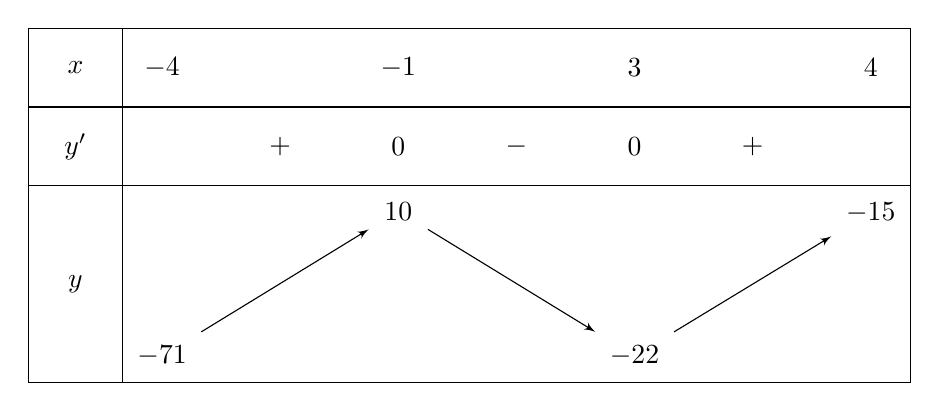
\begin{tikzpicture}[>=stealth]
    % Khởi tạo bảng biến thiên với độ rộng cột tiêu đề và khoảng cách giữa các số
    \tkzTabInit[nocadre=false, lgt=1.2, espcl=3]
        {$x$ / 1, $y'$ / 1, $y$ / 2.5}     % Tên các dòng và chiều cao dòng
        {$-4$, $-1$, $3$, $4$}             % Các giá trị trên dòng x
    
    % Xét dấu của đạo hàm y'
    \tkzTabLine{ , +, 0, -, 0, + }
    
    % Sự biến thiên của hàm số y (mũi tên đi lên/xuống)
    \tkzTabVar{-/ $-71$, +/ $10$, -/ $-22$, +/ $-15$}
\end{tikzpicture}
\end{center}

Giá trị nhỏ nhất của hàm số đã cho trên đoạn \([-4; 4]\) bằng}{
    \begin{tasks}(4)
        \task \(3\)
        \task \(-22\)
        \task \(-71\)
        \task \(-4\)
    \end{tasks}
}

% --- CÂU 22 (tương ứng Câu 5 gốc: THPT Gia Bình) ---
\questionLinesManual{0}{22}{Cho hàm số \( y = f(x) \) liên tục và có bảng biến thiên trên đoạn \([-1; 3]\) như hình vẽ bên. Khẳng định nào đúng?

\begin{center}
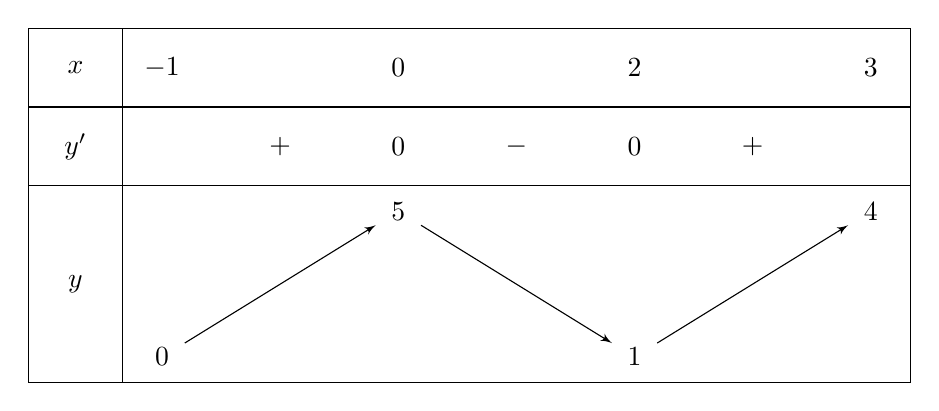
\begin{tikzpicture}[>=stealth]
    % Khởi tạo bảng biến thiên với độ rộng cột tiêu đề và khoảng cách giữa các số
    \tkzTabInit[nocadre=false, lgt=1.2, espcl=3]
        {$x$ / 1, $y'$ / 1, $y$ / 2.5}     % Tên dòng / Chiều cao dòng
        {$-1$, $0$, $2$, $3$}              % Các giá trị trên dòng x
    
    % Xét dấu của đạo hàm y' (+, 0, -, 0, +)
    \tkzTabLine{ , +, 0, -, 0, + }
    
    % Sự biến thiên của hàm số y (mũi tên đi lên/xuống tương ứng với các giá trị cực trị)
    \tkzTabVar{-/ $0$, +/ $5$, -/ $1$, +/ $4$}
\end{tikzpicture}
\end{center}

}{
    \begin{tasks}(4)
        \task \(\min\limits_{[-1; 3]} f(x) = -1\)
        \task \(\min\limits_{[-1; 3]} f(x) = 1\)
        \task \(\max\limits_{[-1; 3]} f(x) = 5\)
        \task \(\max\limits_{[-1; 3]} f(x) = 4\)
    \end{tasks}
}

% --- CÂU 23 (tương ứng Câu 6 gốc: THPT Thạch Thành 1) ---
\questionLinesManual{0}{23}{ Cho hàm số \( y = f(x) \) liên tục và có bảng biến thiên trên đoạn \([-1; 3]\) như hình vẽ bên. Khẳng định nào sau đây là đúng?

\begin{center}
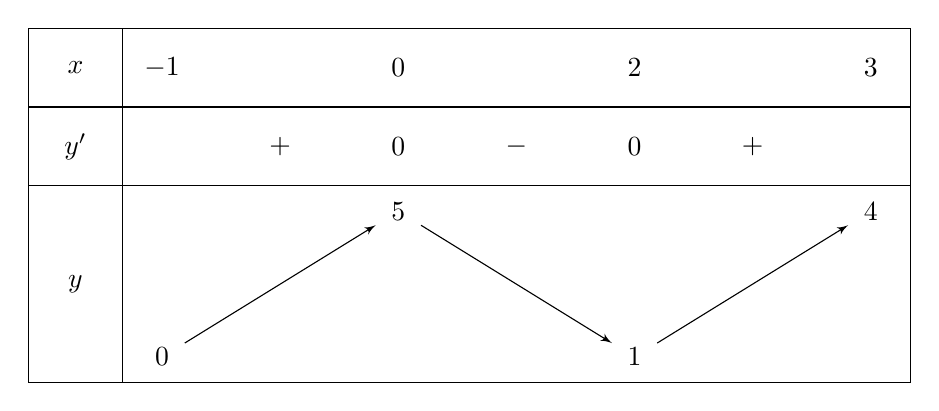
\begin{tikzpicture}[>=stealth]
    % Khởi tạo bảng biến thiên với độ rộng cột tiêu đề và khoảng cách giữa các số
    \tkzTabInit[nocadre=false, lgt=1.2, espcl=3]
        {$x$ / 1, $y'$ / 1, $y$ / 2.5}     % Tên các dòng và chiều cao dòng
        {$-1$, $0$, $2$, $3$}              % Các giá trị trên dòng x
    
    % Điền các dấu và giá trị 0 của đạo hàm y'
    \tkzTabLine{ , +, 0, -, 0, + }
    
    % Điền các mũi tên biến thiên và giá trị cực trị của hàm số y
    \tkzTabVar{-/ $0$, +/ $5$, -/ $1$, +/ $4$}
\end{tikzpicture}
\end{center}

}{
    \begin{tasks}(4)
        \task \( \max\limits_{[-1;3]} f(x) = 4 \)
        \task \( \max\limits_{[-1;3]} f(x) = 5 \)
        \task \( \max\limits_{[-1;3]} f(x) = 1 \)
        \task \( \max\limits_{[-1;3]} f(x) = 0 \)
    \end{tasks}
}

% --- CÂU 24 (tương ứng Câu 9 gốc: THPT Chuyên Vĩnh Phúc) ---
\questionLinesManual{0}{24}{Cho hàm số \( y = f(x) \) có bảng biến thiên trên đoạn \([0; 3]\) như sau.

\begin{center}
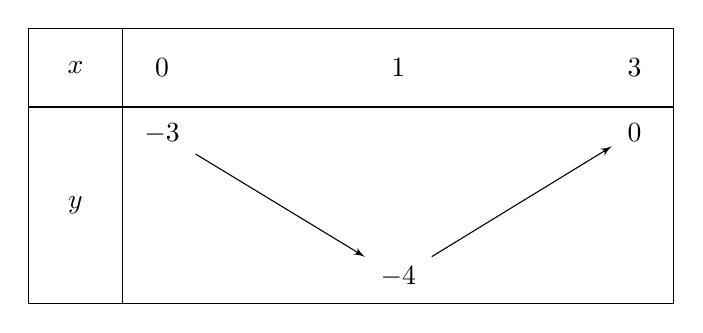
\begin{tikzpicture}[>=stealth]
    % Khởi tạo bảng biến thiên gồm 2 dòng: x và y
    \tkzTabInit[nocadre=false, lgt=1.2, espcl=3]
        {$x$ / 1, $y$ / 2.5}         % Tên các dòng và chiều cao tương ứng
        {$0$, $1$, $3$}              % Các giá trị trên dòng x
    
    % Điền các mũi tên biến thiên và giá trị tương ứng của dòng y
    \tkzTabVar{+/ $-3$, -/ $-4$, +/ $0$}
\end{tikzpicture}
\end{center}

Giá trị nhỏ nhất của hàm số \( y = f(x) \) trên đoạn \([0; 3]\) là}{
    \begin{tasks}(4)
        \task \(-4\)
        \task \(1\)
        \task \(4\)
        \task \(0\)
    \end{tasks}
}

% --- CÂU 25 (tương ứng Câu 12 gốc: THPT Hùng Vương) ---
\questionLinesManual{0}{25}{ Cho hàm số \( y = f(x) \) có bảng biến thiên như sau

\begin{center}
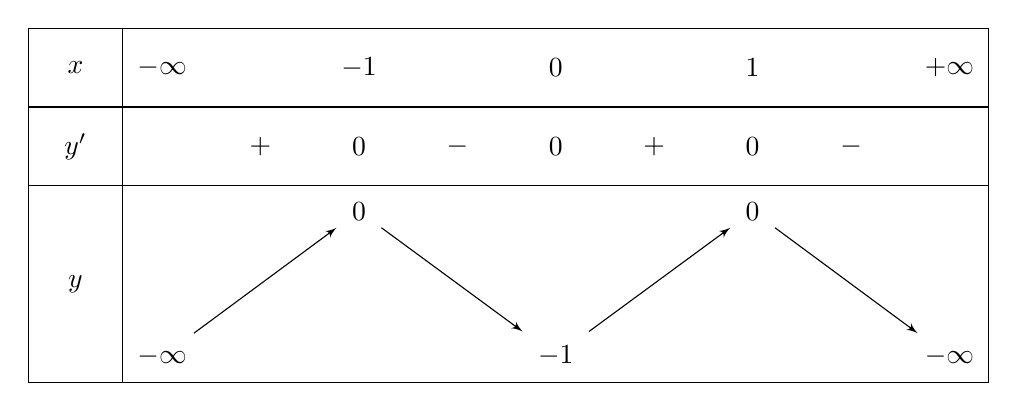
\begin{tikzpicture}[>=stealth]
    % Khởi tạo bảng biến thiên với độ rộng cột tiêu đề và khoảng cách giữa các cột số
    \tkzTabInit[nocadre=false, lgt=1.2, espcl=2.5]
        {$x$ / 1, $y'$ / 1, $y$ / 2.5}                    % Tên dòng / Chiều cao dòng
        {$-\infty$, $-1$, $0$, $1$, $+\infty$}            % Các giá trị trên dòng x
    
    % Xét dấu của đạo hàm y' (+, 0, -, 0, +, 0, -)
    \tkzTabLine{ , +, 0, -, 0, +, 0, - }
    
    % Sự biến thiên và các giá trị cực trị của hàm số y
    \tkzTabVar{-/ $-\infty$, +/ $0$, -/ $-1$, +/ $0$, -/ $-\infty$}
\end{tikzpicture}
\end{center}

Khẳng định nào sau đây sai?}{
    \begin{tasks}(1)
        \task Hàm số \( y = f(x) \) nghịch biến trên \((-1; 0)\) và \((1; +\infty)\).
        \task Giá trị nhỏ nhất của hàm số \( y = f(x) \) trên tập \( \mathbb{R} \) bằng \(-1\).
        \task Giá trị lớn nhất của hàm số \( y = f(x) \) trên tập \( \mathbb{R} \) bằng \(0\).
        \task Đồ thị hàm số \( y = f(x) \) không có đường tiệm cận.
    \end{tasks}
}

% --- CÂU 26 (tương ứng Câu 16 gốc: Sở Hà Tĩnh) ---
\questionLinesManual{0}{26}{ Cho hàm số \( y = f(x) \) có bảng biến thiên như hình bên. Giá trị lớn nhất của hàm số đã cho trên đoạn \([-2; 4]\) bằng

\begin{center}
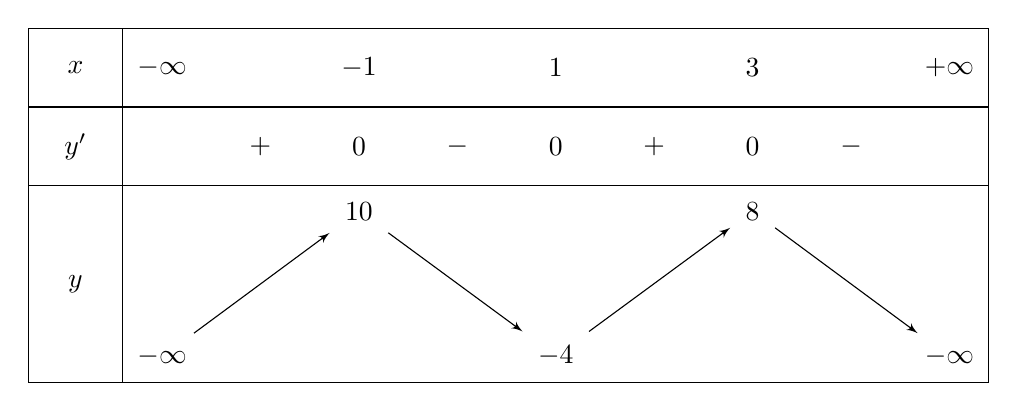
\begin{tikzpicture}[>=stealth]
    % Khởi tạo bảng biến thiên với độ rộng cột tiêu đề và khoảng cách giữa các cột số
    \tkzTabInit[nocadre=false, lgt=1.2, espcl=2.5]
        {$x$ / 1, $y'$ / 1, $y$ / 2.5}                    % Tên dòng / Chiều cao dòng
        {$-\infty$, $-1$, $1$, $3$, $+\infty$}            % Các giá trị trên dòng x
    
    % Xét dấu của đạo hàm y'
    \tkzTabLine{ , +, 0, -, 0, +, 0, - }
    
    % Sự biến thiên và các giá trị cực trị của hàm số y
    \tkzTabVar{-/ $-\infty$, +/ $10$, -/ $-4$, +/ $8$, -/ $-\infty$}
\end{tikzpicture}
\end{center}

}{
    \begin{tasks}(4)
        \task \(-1\)
        \task \(10\)
        \task \(1\)
        \task \(8\)
    \end{tasks}
}

% --- CÂU 27 (tương ứng Câu 18 gốc: Chuyên Thái Bình 2025) ---
\questionLinesManual{0}{27}{ Cho hàm số \( y = f(x) \) liên tục và có bảng biến thiên trên đoạn \([-1; 3]\) như hình vẽ bên.

\begin{center}
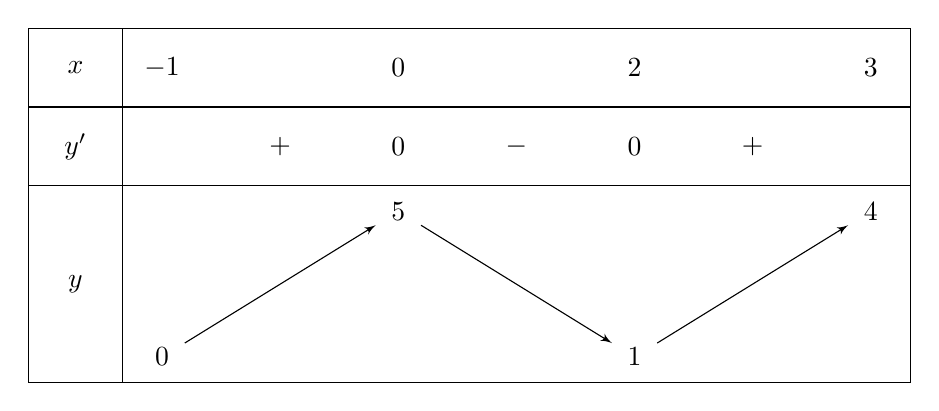
\begin{tikzpicture}[>=stealth]
    % Khởi tạo bảng biến thiên với độ rộng cột tiêu đề và khoảng cách giữa các số
    \tkzTabInit[nocadre=false, lgt=1.2, espcl=3]
        {$x$ / 1, $y'$ / 1, $y$ / 2.5}     % Tên các dòng và chiều cao dòng
        {$-1$, $0$, $2$, $3$}              % Các giá trị trên dòng x
    
    % Xét dấu của đạo hàm y'
    \tkzTabLine{ , +, 0, -, 0, + }
    
    % Sự biến thiên và các giá trị của hàm số y tại các điểm mút và cực trị
    \tkzTabVar{-/ $0$, +/ $5$, -/ $1$, +/ $4$}
\end{tikzpicture}
\end{center}

Khẳng định nào sau đây đúng?}{
    \begin{tasks}(4)
        \task \( \max\limits_{[-1;3]} f(x) = f(0) \)
        \task \( \max\limits_{[-1;3]} f(x) = f(3) \)
        \task \( \max\limits_{[-1;3]} f(x) = f(2) \)
        \task \( \max\limits_{[-1;3]} f(x) = f(-1) \)
    \end{tasks}
}

% --- CÂU 28 (tương ứng Câu 19 gốc: Chuyên Vinh 2025) ---
\questionLinesManual{0}{28}{ Cho hàm số \( y = f(x) \) có bảng xét dấu đạo hàm như sau

\begin{center}
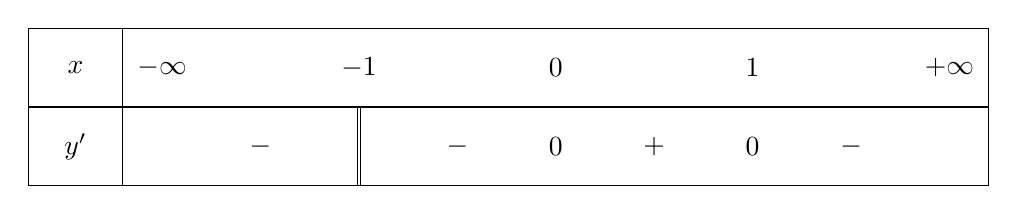
\begin{tikzpicture}[>=stealth]
    % Khởi tạo bảng xét dấu gồm 2 dòng: x và y'
    \tkzTabInit[nocadre=false, lgt=1.2, espcl=2.5]
        {$x$ / 1, $y'$ / 1}                               % Tên dòng / Chiều cao dòng
        {$-\infty$, $-1$, $0$, $1$, $+\infty$}            % Các giá trị trên dòng x
    
    % Xét dấu của đạo hàm y', sử dụng 'd' để tạo dấu hai gạch || tại x = -1
    \tkzTabLine{ , -, d, -, 0, +, 0, - }
\end{tikzpicture}
\end{center}

Mệnh đề nào sau đây đúng?}{
    \begin{tasks}(4)
        \task \(\max\limits_{(0;+\infty)} f(x) = f(1)\)
        \task \(\max\limits_{[-1;1]} f(x) = f(0)\)
        \task \(\max\limits_{(-\infty;-1]} f(x) = f(-1)\)
        \task \(\min\limits_{(0;1]} f(x) = f(0)\)
    \end{tasks}
}

% --- CÂU 29 (tương ứng Câu 28 gốc: Chuyên Hùng Vương) ---
\questionLinesManual{0}{29}{ Cho hàm số \( y = f(x) \) xác định trên \( \mathbb{R} \) và có bảng xét dấu \( f'(x) \) như sau:

\begin{center}
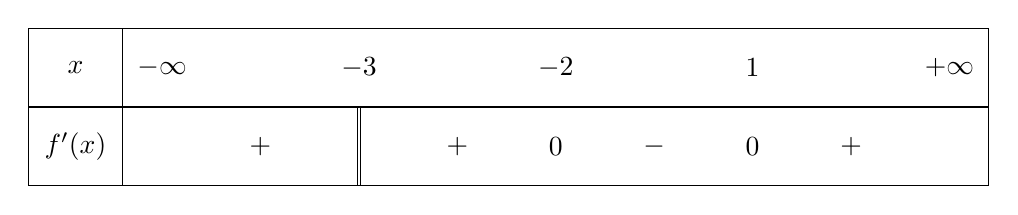
\begin{tikzpicture}[>=stealth]
    % Khởi tạo bảng xét dấu gồm 2 dòng: x và f'(x)
    \tkzTabInit[nocadre=false, lgt=1.2, espcl=2.5]
        {$x$ / 1, $f'(x)$ / 1}                            % Tên dòng / Chiều cao dòng
        {$-\infty$, $-3$, $-2$, $1$, $+\infty$}           % Các giá trị trên dòng x
    
    % Xét dấu của đạo hàm f'(x), sử dụng 'd' tại x = -3
    \tkzTabLine{ , +, d, +, 0, -, 0, + }
\end{tikzpicture}
\end{center}

Khẳng định nào dưới đây đúng?}{
    \begin{tasks}(4)
        \task \(\min\limits_{(-2;+\infty)} f(x) = f(1)\)
        \task \(\min\limits_{(-\infty;-3]} f(x) = f(-3)\)
        \task \(\min\limits_{[-2;1]} f(x) = f(1)\)
        \task \(\min\limits_{[-3;-2]} f(x) = f(-2)\)
    \end{tasks}
}

% --- CÂU 30 (tương ứng Câu 36 gốc: THPT Triệu Quang Phục) ---
\questionLinesManual{0}{30}{ Cho hàm số \( y = f(x) \) liên tục trên đoạn \([-4; 3]\), có bảng biến thiên như hình vẽ. Khẳng định nào sau đây là đúng?

\begin{center}
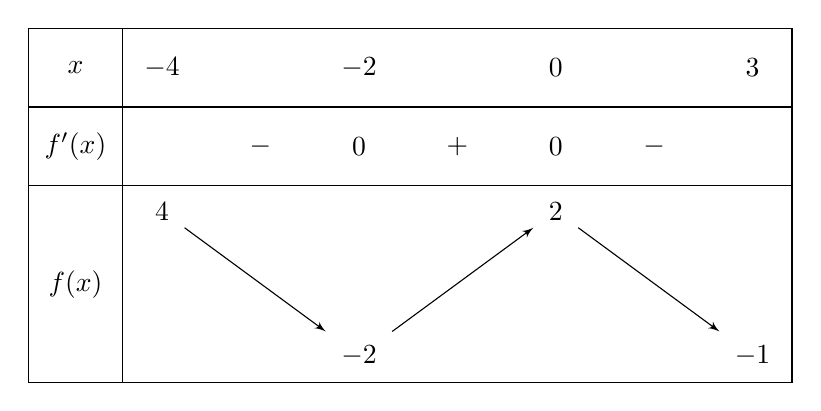
\begin{tikzpicture}[>=stealth]
    % Khởi tạo bảng biến thiên với độ rộng cột tiêu đề và khoảng cách giữa các cột số
    \tkzTabInit[nocadre=false, lgt=1.2, espcl=2.5]
        {$x$ / 1, $f'(x)$ / 1, $f(x)$ / 2.5}         % Tên dòng / Chiều cao dòng
        {$-4$, $-2$, $0$, $3$}                       % Các giá trị trên dòng x
    
    % Xét dấu của đạo hàm f'(x)
    \tkzTabLine{ , -, 0, +, 0, - }
    
    % Sự biến thiên và các giá trị cực trị của hàm số f(x)
    \tkzTabVar{+/ $4$, -/ $-2$, +/ $2$, -/ $-1$}
\end{tikzpicture}
\end{center}

}{
    \begin{tasks}(4)
        \task \( \min\limits_{[-4;3]} f(x) = -1 \) tại \( x = 3 \)
        \task \( \max\limits_{[-4;3]} f(x) = 4 \) tại \( x = -4 \)
        \task \( \max\limits_{[-4;3]} f(x) = 2 \) tại \( x = 0 \)
        \task \( \min\limits_{[-4;3]} f(x) = -2 \) tại \( x = 2 \)
    \end{tasks}
}

% --- CÂU 31 (tương ứng Câu 41 gốc: Sở Hà Tĩnh) ---
\questionLinesManual{0}{31}{Cho hàm số \( y = f(x) \) có bảng biến thiên trên đoạn \([0; 3]\) như sau:

\begin{center}
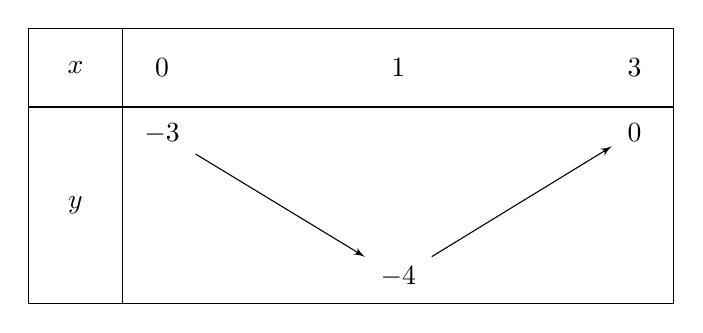
\begin{tikzpicture}[>=stealth]
    % Khởi tạo bảng biến thiên gồm 2 dòng: x và y
    \tkzTabInit[nocadre=false, lgt=1.2, espcl=3]
        {$x$ / 1, $y$ / 2.5}         % Tên các dòng và chiều cao tương ứng
        {$0$, $1$, $3$}              % Các giá trị trên dòng x
    
    % Điền các mũi tên biến thiên và giá trị tương ứng của dòng y
    \tkzTabVar{+/ $-3$, -/ $-4$, +/ $0$}
\end{tikzpicture}
\end{center}

Giá trị nhỏ nhất của hàm số \( y = f(x) \) trên đoạn \([0; 3]\) là}{
    \begin{tasks}(4)
        \task \(-4\)
        \task \(1\)
        \task \(4\)
        \task \(0\)
    \end{tasks}
}

% --- CÂU 32 (tương ứng Câu 2 gốc: Đề Minh Họa 2017) ---
\questionLinesManual{0}{32}{ Cho hàm số \( y = f(x) \) xác định, liên tục trên \( \mathbb{R} \) và có bảng biến thiên:

\begin{center}
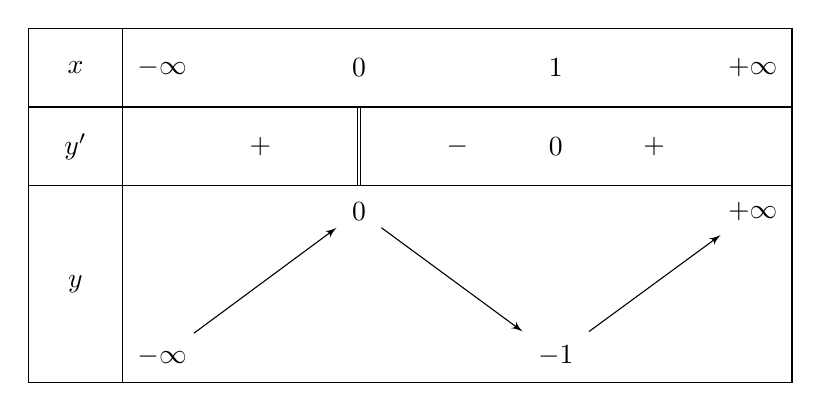
\begin{tikzpicture}[>=stealth]
    % Khởi tạo bảng biến thiên với độ rộng cột tiêu đề và khoảng cách giữa các số
    \tkzTabInit[nocadre=false, lgt=1.2, espcl=2.5]
        {$x$ / 1, $y'$ / 1, $y$ / 2.5}                    % Tên dòng / Chiều cao dòng
        {$-\infty$, $0$, $1$, $+\infty$}                  % Các giá trị trên dòng x
    
    % Xét dấu của đạo hàm y', sử dụng 'd' tại x = 0
    \tkzTabLine{ , +, d, -, 0, + }
    
    % Sự biến thiên và các giá trị của hàm số y
    \tkzTabVar{-/ $-\infty$, +/ $0$, -/ $-1$, +/ $+\infty$}
\end{tikzpicture}
\end{center}

Khẳng định nào sau đây là khẳng định đúng?}{
    \begin{tasks}(1)
        \task Hàm số có giá trị cực tiểu bằng 1.
        \task Hàm số có giá trị lớn nhất bằng 0 và giá trị nhỏ nhất bằng \(-1\).
        \task Hàm số đạt cực đại tại \( x = 0 \) và đạt cực tiểu tại \( x = 1 \).
        \task Hàm số có đúng một cực trị.
    \end{tasks}
}

% --- CÂU 33 (tương ứng Câu 2 gốc thứ hai) ---
\questionLinesManual{0}{33}{Cho hàm số \( y = f(x) \) liên tục trên \([-3; 2]\) và có bảng biến thiên như sau. Gọi \( M, m \) lần lượt là giá trị lớn nhất và giá trị nhỏ nhất của hàm số \( y = f(x) \) trên đoạn \([-1; 2]\). Tính \( M + m \).

\begin{center}
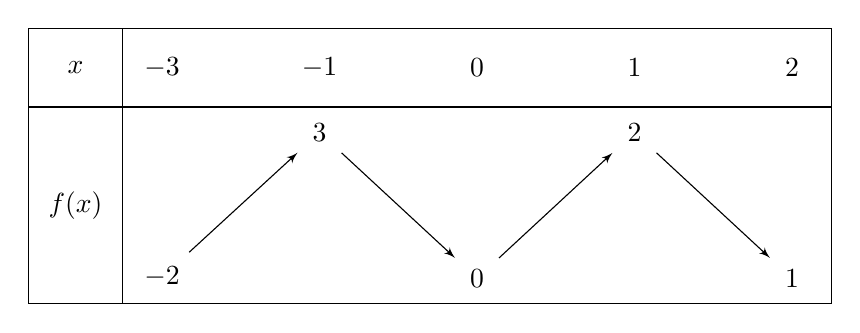
\begin{tikzpicture}[>=stealth]
    % Khởi tạo bảng biến thiên gồm 2 dòng: x và f(x)
    \tkzTabInit[nocadre=false, lgt=1.2, espcl=2]
        {$x$ / 1, $f(x)$ / 2.5}                   % Tên các dòng và chiều cao tương ứng
        {$-3$, $-1$, $0$, $1$, $2$}               % Các giá trị trên dòng x
    
    % Điền các mũi tên biến thiên và giá trị của hàm số f(x)
    \tkzTabVar{-/ $-2$, +/ $3$, -/ $0$, +/ $2$, -/ $1$}
\end{tikzpicture}
\end{center}

}{
    \begin{tasks}(4)
        \task $3$
        \task $2$
        \task $1$
        \task $4$
    \end{tasks}
}

% --- CÂU 34 (tương ứng Câu 6 gốc: THPT Ba Đình) ---
\questionLinesManual{0}{34}{ Xét hàm số \( y = f(x) \) với \( x \in [-1; 5] \) có bảng biến thiên như sau:

\begin{center}
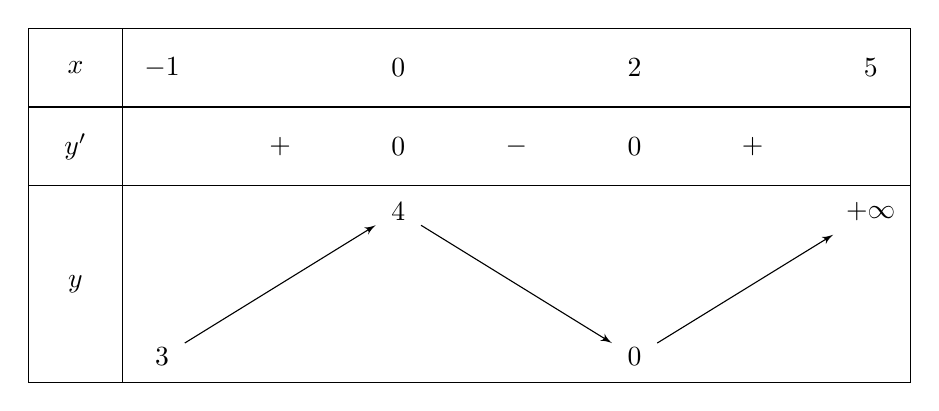
\begin{tikzpicture}[>=stealth]
    % Khởi tạo bảng biến thiên với độ rộng cột tiêu đề và khoảng cách giữa các số
    \tkzTabInit[nocadre=false, lgt=1.2, espcl=3]
        {$x$ / 1, $y'$ / 1, $y$ / 2.5}         % Tên các dòng và chiều cao dòng
        {$-1$, $0$, $2$, $5$}                  % Các giá trị trên dòng x
    
    % Xét dấu của đạo hàm y'
    \tkzTabLine{ , +, 0, -, 0, + }
    
    % Điền các mũi tên biến thiên và giá trị tương ứng của hàm số y
    \tkzTabVar{-/ $3$, +/ $4$, -/ $0$, +/ $+\infty$}
\end{tikzpicture}
\end{center}

Khẳng định nào sau đây là đúng}{
    \begin{tasks}(1)
        \task Hàm số đã cho không tồn tại GTLN trên đoạn \([-1; 5]\)
        \task Hàm số đã cho đạt GTNN tại \( x = -1 \) và \( x = 2 \) trên đoạn \([-1; 5]\)
        \task Hàm số đã cho đạt GTNN tại \( x = -1 \) và đạt GTLN tại \( x = 5 \) trên đoạn \([-1; 5]\)
        \task Hàm số đã cho đạt GTNN tại \( x = 0 \) trên đoạn \([-1; 5]\)
    \end{tasks}
}

% --- CÂU 35 (tương ứng Câu 7 gốc: Chuyên Lê Thánh Tông) ---
\questionLinesManual{0}{35}{ Cho hàm số \( y = f(x) \) liên tục trên \( \mathbb{R} \), có bảng biến thiên như hình sau:

\begin{center}
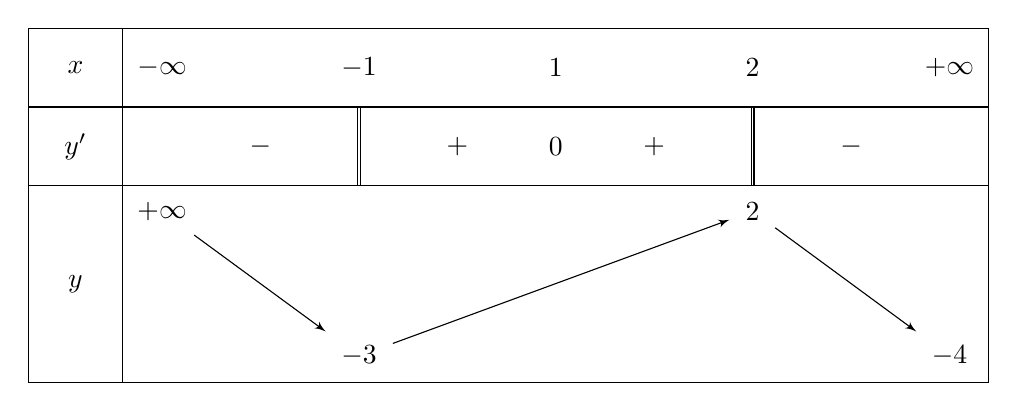
\begin{tikzpicture}[>=stealth]
    % Khởi tạo bảng biến thiên với độ rộng cột tiêu đề và khoảng cách giữa các số
    \tkzTabInit[nocadre=false, lgt=1.2, espcl=2.5]
        {$x$ / 1, $y'$ / 1, $y$ / 2.5}                   % Tên dòng / Chiều cao dòng
        {$-\infty$, $-1$, $1$, $2$, $+\infty$}           % Các giá trị trên dòng x
    
    % Xét dấu của đạo hàm y'
    % Sử dụng 'd' tại x = -1 và x = 2 để tạo vạch kép ||
    \tkzTabLine{ , -, d, +, 0, +, d, - }
    
    % Sự biến thiên và các giá trị của hàm số y
    % Sử dụng 'R/' tại x = 1 để mũi tên nối thẳng từ -3 lên 2
    \tkzTabVar{+/ $+\infty$, -/ $-3$, R/, +/ $2$, -/ $-4$}
\end{tikzpicture}
\end{center}

Trong các mệnh đề sau, mệnh đề nào sai?}{
    \begin{tasks}(1)
        \task Hàm số có hai điểm cực trị.
        \task Hàm số có giá trị lớn nhất bằng 2 và giá trị nhỏ nhất bằng -3.
        \task Đồ thị hàm số có đúng một đường tiệm cận.
        \task Hàm số nghịch biến trên mỗi khoảng \((-\infty; -1)\), \((2; +\infty)\).
    \end{tasks}
}

% --- CÂU 36 (tương ứng Câu 8 gốc: Chuyên Nguyễn Tất Thành Yên Bái) ---
\questionLinesManual{0}{36}{ Cho hàm số \( y = f(x) \) liên tục và có bảng biến thiên trên đoạn \([-1; 3]\) như hình vẽ bên. Khẳng định nào sau đây đúng?

\begin{center}
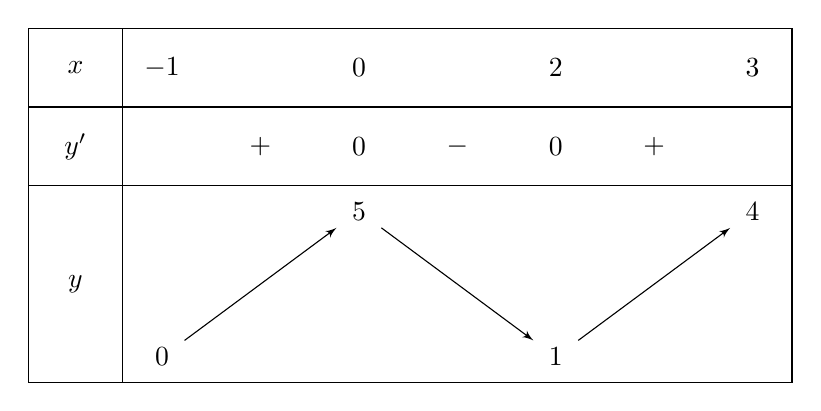
\begin{tikzpicture}[>=stealth]
    % Khởi tạo bảng biến thiên với độ rộng cột tiêu đề và khoảng cách giữa các số
    \tkzTabInit[nocadre=false, lgt=1.2, espcl=2.5]
        {$x$ / 1, $y'$ / 1, $y$ / 2.5}         % Tên các dòng và chiều cao tương ứng
        {$-1$, $0$, $2$, $3$}                  % Các giá trị trên dòng x
    
    % Xét dấu của đạo hàm y'
    \tkzTabLine{ , +, 0, -, 0, + }
    
    % Điền các mũi tên biến thiên và giá trị tương ứng của hàm số y
    \tkzTabVar{-/ $0$, +/ $5$, -/ $1$, +/ $4$}
\end{tikzpicture}
\end{center}

}{
    \begin{tasks}(1)
        \task \(\max\limits_{[-1;3]} f(x) = f(0)\)
        \task \(\max\limits_{[-1;3]} f(x) = f(3)\)
        \task \(\max\limits_{[-1;3]} f(x) = f(2)\)
        \task \(\max\limits_{[-1;3]} f(x) = f(-1)\)
    \end{tasks}
}

% --- CÂU 37 (tương ứng Câu 4 gốc: THPT Nguyễn Đăng Đạo) ---
\questionLinesManual{0}{37}{ Gọi \( M, m \) lần lượt là giá trị lớn nhất và giá trị nhỏ nhất của hàm số \( f(x) = x^4 - 2x^2 - 1 \) trên đoạn \([-1; 2]\). Giá trị của biểu thức \( M + 3m \) bằng}{
    \begin{tasks}(4)
        \task $1$
        \task $5$
        \task $6$
        \task $4$
    \end{tasks}
}

% --- CÂU 38 (tương ứng Câu 7 gốc: THPT Thạch Thành 1) ---
\questionLinesManual{0}{38}{ Giá trị lớn nhất của hàm số \( f(x) = x^3 - 3x^2 - 9x + 10 \) trên đoạn \([-2; 2]\) bằng:}{
    \begin{tasks}(4)
        \task $-12$
        \task $10$
        \task $15$
        \task $-2$
    \end{tasks}
}

% --- CÂU 39 (tương ứng Câu 10 gốc: THPT Nguyễn Viết Xuân) ---
\questionLinesManual{0}{39}{(THPT Nguyễn Viết Xuân - Vĩnh Phúc 2025) Giá trị nhỏ nhất của hàm số \( y = x^3 + 3x - 6 \) trên đoạn \([1; 3]\) là:}{
    \begin{tasks}(4)
        \task $-39$
        \task $-2$
        \task $-10$
        \task $-6$
    \end{tasks}
}

% --- CÂU 40 (tương ứng Câu 11 gốc: THPT Thuận Thành 1&2) ---
\questionLinesManual{0}{40}{Giá trị lớn nhất của hàm số \( y = x^3 - 3x + 1 \) trên đoạn \([-2; 0]\)}{
    \begin{tasks}(4)
        \task $1$
        \task $3$
        \task $-1$
        \task $2$
    \end{tasks}
}

% --- CÂU 41 (tương ứng Câu 14 gốc: THPT Triệu Sơn 1) ---
\questionLinesManual{0}{41}{ Giá trị nhỏ nhất của hàm số \( f(x) = x^3 - 3x + 2 \) trên đoạn \([-3; 3]\) bằng}{
    \begin{tasks}(4)
        \task $0$
        \task $-16$
        \task $4$
        \task $20$
    \end{tasks}
}

% --- CÂU 42 (tương ứng Câu 15 gốc: THPT Cụm trường Hải Dương) ---
\questionLinesManual{0}{42}{ Giá trị nhỏ nhất của hàm số \( f(x) = x^3 - 6x^2 + 9x - 1 \) trên nửa khoảng \([-1; +\infty)\) là}{
    \begin{tasks}(4)
        \task $1$
        \task $-17$
        \task $17$
        \task $3$
    \end{tasks}
}

% --- CÂU 43 (tương ứng Câu 20 gốc: THPT Cẩm Xuyên) ---
\questionLinesManual{0}{43}{ Giá trị lớn nhất của hàm số \( f(x) = x^3 + 3x - 6 \) trên đoạn \([1; 3]\) là}{
    \begin{tasks}(4)
        \task $30$
        \task $39$
        \task $36$
        \task $10$
    \end{tasks}
}

% --- CÂU 44 (tương ứng Câu 22 gốc: THPT Sào Nam) ---
\questionLinesManual{0}{44}{ Giá trị nhỏ nhất của hàm số \( f(x) = -x^3 - x + 2 \) trên đoạn \([-2; 0]\) bằng?}{
    \begin{tasks}(4)
        \task $2$
        \task $-2$
        \task $0$
        \task $-8$
    \end{tasks}
}

% --- CÂU 45 (tương ứng Câu 23 gốc: Cụm trường Nguyễn Hiền - Lê Hồng Phong) ---
\questionLinesManual{0}{45}{ Giá trị lớn nhất của hàm số \( f(x) = -x^4 + 12x^2 + 1 \) trên đoạn \([-1; 2]\) bằng}{
    \begin{tasks}(4)
        \task $37$
        \task $1$
        \task $12$
        \task $33$
    \end{tasks}
}

% --- CÂU 46 (tương ứng Câu 24 gốc: THPT Nông Cống 3) ---
\questionLinesManual{0}{46}{ Tìm giá trị nhỏ nhất của hàm số \( y = -x + 3 - \dfrac{1}{x + 2} \) trên nửa khoảng \([-4; -2)\).}{
    \begin{tasks}(4)
        \task \( \min\limits_{[-4; -2)} y = 5 \)
        \task \( \min\limits_{[-4; -2)} y = 4 \)
        \task \( \min\limits_{[-4; -2)} y = 7 \)
        \task \( \min\limits_{[-4; -2)} y = \dfrac{15}{2} \)
    \end{tasks}
}

% --- CÂU 47 (tương ứng Câu 25 gốc: THPT Anh Sơn 3) ---
\questionLinesManual{0}{47}{Giá trị lớn nhất của hàm số \( f(x) = x^3 - 3x^2 - 9x + 10 \) trên đoạn \([-2; 2]\) là}{
    \begin{tasks}(4)
        \task $17$
        \task $10$
        \task $15$
        \task $-12$
    \end{tasks}
}

% --- CÂU 48 (tương ứng Câu 26 gốc: Sở Bắc Giang) ---
\questionLinesManual{0}{48}{ Giá trị nhỏ nhất của hàm số \( y = x^4 - 4x^2 + 3 \) trên đoạn \([0; 4]\) là}{
    \begin{tasks}(4)
        \task $0$
        \task $\sqrt{2}$
        \task $3$
        \task $-1$
    \end{tasks}
}

% --- CÂU 49 (tương ứng Câu 27 gốc: Sở Thái Nguyên) ---
\questionLinesManual{0}{49}{ Giá trị lớn nhất của hàm số \( y = x^3 - 3x + 4 \) trên đoạn \([-2; 0]\) bằng}{
    \begin{tasks}(4)
        \task $2$
        \task $4$
        \task $12$
        \task $6$
    \end{tasks}
}

% --- CÂU 50 (tương ứng Câu 31 gốc: Liên Trường Nghệ An) ---
\questionLinesManual{0}{50}{ Tìm giá trị lớn nhất \( M \) của hàm số \( y = x^3 + 3x^2 - 9x - 6 \) trên đoạn \([-1; 2]\).}{
    \begin{tasks}(4)
        \task \( M = 21 \)
        \task \( M = 7 \)
        \task \( M = 5 \)
        \task \( M = -11 \)
    \end{tasks}
}

% --- CÂU 51 (tương ứng Câu 33 gốc: Cụm Ninh Giang - Tứ Kỳ - Gia Lộc) ---
\questionLinesManual{0}{51}{ Giá trị lớn nhất \( M \) của hàm số \( y = x^3 + 3x^2 - 9x - 6 \) trên đoạn \([-1; 2]\) là?}{
    \begin{tasks}(4)
        \task \( M = 7 \)
        \task \( M = 5 \)
        \task \( M = -11 \)
        \task \( M = 21 \)
    \end{tasks}
}

% --- CÂU 52 (tương ứng Câu 35 gốc: THPT Mai Trúc Loan) ---
\questionLinesManual{0}{52}{Giá trị lớn nhất của hàm số \( y = x^3 - 3x \) trên đoạn \([0; 3]\) bằng}{
    \begin{tasks}(4)
        \task $2$
        \task $18$
        \task $-2$
        \task $0$
    \end{tasks}
}

% --- CÂU 53 (tương ứng Câu 40 gốc: THPT Bắc Đông Quan) ---
\questionLinesManual{0}{53}{ Gọi \( M, m \) lần lượt là giá trị lớn nhất và giá trị nhỏ nhất của hàm số \( y = 2 - \sin x \). Khẳng định nào sau đây đúng?}{
    \begin{tasks}(4)
        \task \( M = 2; m = 1 \)
        \task \( M = 1; m = -1 \)
        \task \( M = 3; m = 0 \)
        \task \( M = 3; m = 1 \)
    \end{tasks}
}

% --- CÂU 54 (tương ứng Câu 17 gốc: Chuyên Bắc Ninh 2018) ---
\questionLinesManual{0}{54}{Tìm tập giá trị của hàm số \( y = \sqrt{x - 1} + \sqrt{9 - x} \)}{
    \begin{tasks}(4)
        \task \( T = [1; 9] \)
        \task \( T = [2\sqrt{2}; 4] \)
        \task \( T = (1; 9) \)
        \task \( T = [0; 2\sqrt{2}] \)
    \end{tasks}
}

% --- CÂU 55 (tương ứng Câu 28 gốc: Sở Nam Định 2019) ---
\questionLinesManual{0}{55}{Giá trị lớn nhất của hàm số \( y = \sqrt{4 - x^2} \) là}{
    \begin{tasks}(4)
        \task $2$
        \task $0$
        \task $4$
        \task $1$
    \end{tasks}
}

% --- CÂU 56 (tương ứng Câu 29 gốc: Chuyên Bắc Ninh 2018) ---
\questionLinesManual{0}{56}{Tìm giá trị nhỏ nhất của hàm số \( y = \sin^2 x - 4 \sin x - 5 \).}{
    \begin{tasks}(4)
        \task $-20$
        \task $-8$
        \task $-9$
        \task $0$
    \end{tasks}
}

% --- CÂU 57 (tương ứng Câu 30 gốc: THPT Hoa Lư A 2018) ---
\questionLinesManual{0}{57}{ Gọi \( m, M \) lần lượt là giá trị nhỏ nhất và giá trị lớn nhất của hàm số \( f(x) = \dfrac{1}{2}x - \sqrt{x + 1} \) trên đoạn \([0; 3]\). Tính tổng \( S = 2m + 3M \).}{
    \begin{tasks}(4)
        \task \( S = -\dfrac{7}{2} \)
        \task \( S = -\dfrac{3}{2} \)
        \task $-3$
        \task \( S = 4 \)
    \end{tasks}
}

% --- CÂU 58 (tương ứng Câu 31 gốc: Chuyên ĐHSPHN 2018) ---
\questionLinesManual{0}{58}{ Tìm giá trị lớn nhất của hàm số \( f(x) = \sin x + \cos 2x \) trên \([0; \pi]\) là}{
    \begin{tasks}(4)
        \task \(\dfrac{9}{8}\)
        \task \(\dfrac{5}{4}\)
        \task $2$
        \task $1$
    \end{tasks}
}

% --- CÂU 59 (tương ứng Câu 32 gốc: THPT Hà Huy Tập 2018) ---
\questionLinesManual{0}{59}{Giá trị lớn nhất của hàm số \( y = 2 \cos x - \dfrac{4}{3} \cos^3 x \) trên \([0; \pi]\).}{
    \begin{tasks}(4)
        \task \(\max\limits_{[0; \pi]} y = \dfrac{2}{3}\)
        \task \(\max\limits_{[0; \pi]} y = \dfrac{10}{3}\)
        \task \(\max\limits_{[0; \pi]} y = \dfrac{2\sqrt{2}}{3}\)
        \task \(\max\limits_{[0; \pi]} y = 0\)
    \end{tasks}
}

% --- CÂU 60 (tương ứng Câu 33 gốc) ---
\questionLinesManual{0}{60}{Gọi \( M, m \) lần lượt là giá trị lớn nhất và giá trị nhỏ nhất của hàm số \( y = \dfrac{3 \sin x + 2}{\sin x + 1} \) trên đoạn \(\left[ 0; \dfrac{\pi}{2} \right]\). Khi đó giá trị của \( M^2 + m^2 \) là}{
    \begin{tasks}(4)
        \task \(\dfrac{31}{2}\)
        \task \(\dfrac{11}{2}\)
        \task \(\dfrac{41}{4}\)
        \task \(\dfrac{61}{4}\)
    \end{tasks}
}

% --- CÂU 61 (tương ứng Câu 1 gốc: Đề Tham Khảo 2017) ---
\questionLinesManual{0}{61}{ Tính giá trị nhỏ nhất của hàm số \( y = 3x + \dfrac{4}{x^2} \) trên khoảng \( (0; +\infty) \).}{
    \begin{tasks}(4)
        \task \( \min\limits_{(0;+\infty)} y = \dfrac{33}{5} \)
        \task \( \min\limits_{(0;+\infty)} y = 2\sqrt[3]{9} \)
        \task \( \min\limits_{(0;+\infty)} y = 3\sqrt[3]{9} \)
        \task \( \min\limits_{(0;+\infty)} y = 7 \)
    \end{tasks}
}

% --- CÂU 62 (tương ứng Câu 2 gốc) ---
\questionLinesManual{0}{62}{Gọi \( m \) là giá trị nhỏ nhất của hàm số \( y = x - 1 + \dfrac{4}{x - 1} \) trên khoảng \( (1; +\infty) \). Tìm \( m \)?}{
    \begin{tasks}(4)
        \task \( m = 5 \)
        \task \( m = 4 \)
        \task \( m = 2 \)
        \task \( m = 3 \)
    \end{tasks}
}

% --- CÂU 63 (tương ứng Câu 3 gốc: THPT Minh Châu Hưng Yên 2019) ---
\questionLinesManual{0}{63}{ Giá trị nhỏ nhất của hàm số \( y = x - 5 + \dfrac{1}{x} \) trên khoảng \( (0; +\infty) \) bằng bao nhiêu?}{
    \begin{tasks}(4)
        \task $0$
        \task $-1$
        \task $-3$
        \task $-2$
    \end{tasks}
}

% --- CÂU 64 (tương ứng Câu 4 gốc: Chuyên Lương Thế Vinh Đồng Nai 2019) ---
\questionLinesManual{0}{64}{ Gọi \( m \) là giá trị nhỏ nhất của hàm số \( y = x + \dfrac{4}{x} \) trên khoảng \( (0; +\infty) \). Tìm \( m \)}{
    \begin{tasks}(4)
        \task \( m = 4 \)
        \task \( m = 2 \)
        \task \( m = 1 \)
        \task \( m = 3 \)
    \end{tasks}
}

% --- CÂU 65 (tương ứng Câu 5 gốc: Chuyên Bắc Giang 2019) ---
\questionLinesManual{0}{65}{ Giá trị nhỏ nhất của hàm số \( f(x) = x + \dfrac{1}{x} \) trên nửa khoảng \( [2; +\infty) \) là:}{
    \begin{tasks}(4)
        \task $2$
        \task $\dfrac{5}{2}$
        \task $0$
        \task $\dfrac{7}{2}$
    \end{tasks}
}
% --- CÂU 66: ĐỒ THỊ HÀM SỐ y = f(x) ---
\questionTrueFalse{0}{66}{Sử dụng đồ thị hàm số \( y = f(x) \) (hình bên)

\begin{center}
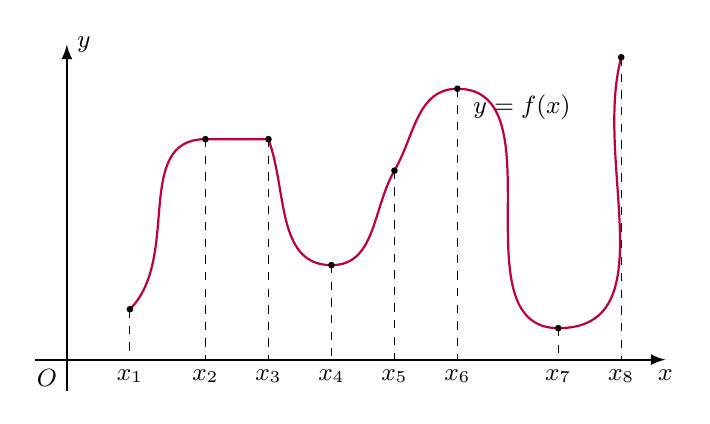
\begin{tikzpicture}[>=latex, scale=0.8]
    % 1. Hệ trục tọa độ Ox, Oy màu đen
    \draw[->, black, thick] (-0.5, 0) -- (9.5, 0) node[below] {\small $x$};
    \draw[->, black, thick] (0, -0.5) -- (0, 5) node[right] {\small $y$};
    \node[below left] at (0, 0) {\small $O$};

    % Khai báo các điểm tọa độ cực trị và điểm uốn (tương đối theo hình)
    \coordinate (P1) at (1, 0.8);
    \coordinate (P2) at (2.2, 3.5);
    \coordinate (P3) at (3.2, 3.5);
    \coordinate (P4) at (4.2, 1.5);
    \coordinate (P5) at (5.2, 3);
    \coordinate (P6) at (6.2, 4.3);
    \coordinate (P7) at (7.8, 0.5);
    \coordinate (P8) at (8.8, 4.8);

    % 2. Đồ thị hàm số y = f(x) màu tím (Purple)
    % Sử dụng to[out=..., in=...] để tạo đường cong mượt đi qua các điểm
    \draw[purple, thick] 
        (P1) to[out=45, in=180] (P2)      
        -- (P3)                           
        to[out=-70, in=180] (P4)          
        to[out=0, in=240] (P5)            
        to[out=60, in=180] (P6)           
        to[out=0, in=180] (P7)            
        to[out=0, in=255] (P8);           

    % 3. Các đường nét đứt, điểm đen và nhãn tọa độ màu đen
    \foreach \i/\p in {1/P1, 2/P2, 3/P3, 4/P4, 5/P5, 6/P6, 7/P7, 8/P8} {
        \draw[dashed, black] (\p) -- (\p |- 0,0);
        \node[below] at (\p |- 0,0) {\small $x_\i$};
        \fill[black] (\p) circle (1.5pt);
    }

    % 4. Thêm nhãn tên hàm số
    \node[right] at (6.3, 4) {\small $y=f(x)$};

\end{tikzpicture}
\end{center}

Xét tính đúng sai của các mệnh đề sau}{
    \textbf{a)} & Hàm số đạt giá trị lớn nhất tại điểm \( x_8 \).
    & \textcolor{amberorange}{$\bigcirc$} & \textcolor{amberorange}{$\bigcirc$} \\ \hline
    
    \textbf{b)} & Hàm số đạt giá trị nhỏ nhất tại điểm \( x_7 \).
    & \textcolor{amberorange}{$\bigcirc$} & \textcolor{amberorange}{$\bigcirc$} \\ \hline
    
    \textbf{c)} & Hàm số đạt cực đại tại điểm \( x_6 \).
    & \textcolor{amberorange}{$\bigcirc$} & \textcolor{amberorange}{$\bigcirc$} \\ \hline
    
    \textbf{d)} & Hàm số đạt cực tiểu tại các điểm \( x_4 \) và \( x_7 \).
    & \textcolor{amberorange}{$\bigcirc$} & \textcolor{amberorange}{$\bigcirc$} \\
}

% --- CÂU 2: ĐỒ THỊ HÀM SỐ y = g(x) GHÉP TỪ 3 ĐỒ THỊ ---
\questionTrueFalse{0}{67}{Cho hàm số \( y = g(x) \) liên tục trên đoạn \([-3; 3]\) và có đồ thị như hình vẽ. Xét tính đúng sai của các mệnh đề sau

\begin{center}
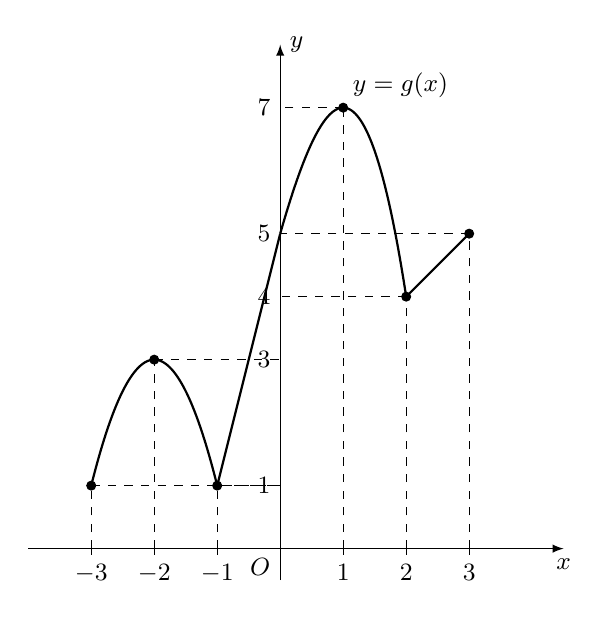
\begin{tikzpicture}[>=latex, scale=0.8]
    % 1. Hệ trục tọa độ
    \draw[->] (-4,0) -- (4.5,0) node[below] {\small $x$};
    \draw[->] (0,-0.5) -- (0,8) node[right] {\small $y$};
    \node[below left] at (0,0) {\small $O$};
    
    % 2. Đánh dấu các mốc trên trục x
    \foreach \x in {-3,-2,-1,1,2,3} {
        \draw (\x,0.1) -- (\x,-0.1) node[below] {\small $\x$};
    }
    
    % 3. Vẽ đồ thị hàm số g(x)
    % Nhánh 1: Parabol y = -2(x+2)^2 + 3 trên [-3, -1]
    \draw[thick, black, samples=100, domain=-3:-1] 
        plot (\x, {-2*(\x+2)^2 + 3});
    
    % Nhánh 2: Parabol y = -3(x-1)^2 + 7 trên [0, 2]
    \draw[thick, black, samples=100, domain=0:2] 
      plot (\x, {-1/2*\x^3 - \x^2 + 7/2*\x + 5});
    
    % Nhánh 3: Đoạn thẳng y = x + 2 trên [2, 3]
    \draw[thick, black] (2,4) -- (3,5);
    \draw[thick, black] (-1,1) -- (0,5);
    % 4. Đánh dấu các điểm đặc biệt
    \filldraw (-3,1) circle (2pt);
    \filldraw (-2,3) circle (2pt);
    \filldraw (-1,1) circle (2pt);
    \filldraw (1,7) circle (2pt);
    \filldraw (2,4) circle (2pt);
    \filldraw (3,5) circle (2pt);
    
    % 5. Đường nét đứt gióng xuống trục hoành
    \draw[dashed] (-3,0) -- (-3,1);
    \draw[dashed] (-1,0) -- (-1,1);
    \draw[dashed] (-2,0) -- (-2,3);
    \draw[dashed] (1,0) -- (1,7);
    \draw[dashed] (2,0) -- (2,4);
    \draw[dashed] (3,0) -- (3,5);
    
    % 6. Đường nét đứt gióng sang trục tung
    \draw[dashed] (-3,1) -- (0,1);
    \draw[dashed] (-1,1) -- (0,1);
    \draw[dashed] (-2,3) -- (0,3);
    \draw[dashed] (1,7) -- (0,7);
    \draw[dashed] (2,4) -- (0,4);
    \draw[dashed] (3,5) -- (0,5);
    
    % 7. Nhãn trên trục tung
    \node[left] at (0,1) {\small $1$};
    \node[left] at (0,3) {\small $3$};
    \node[left] at (0,4) {\small $4$};
    \node[left] at (0,5) {\small $5$};
    \node[left] at (0,7) {\small $7$};
    
    % 8. Nhãn hàm số
    \node[above right, font=\small] at (1,7) {$y = g(x)$};
\end{tikzpicture}
\end{center}

}{
    \textbf{a)} & Giá trị lớn nhất của hàm số trên đoạn \([-3; 3]\) bằng 5.
    & \textcolor{amberorange}{$\bigcirc$} & \textcolor{amberorange}{$\bigcirc$} \\ \hline
    
    \textbf{b)} & Trên đoạn \([-3; 3]\), hàm số đạt giá trị lớn nhất tại điểm \(x = 1\).
    & \textcolor{amberorange}{$\bigcirc$} & \textcolor{amberorange}{$\bigcirc$} \\ \hline
    
    \textbf{c)} & Giá trị nhỏ nhất của hàm số trên đoạn \([-3; 3]\) bằng 1.
    & \textcolor{amberorange}{$\bigcirc$} & \textcolor{amberorange}{$\bigcirc$} \\ \hline
    
    \textbf{d)} & Trên đoạn \([-1; 3]\), hàm số đạt giá trị nhỏ nhất tại điểm \(x = 2\).
    & \textcolor{amberorange}{$\bigcirc$} & \textcolor{amberorange}{$\bigcirc$} \\
}
% --- CÂU 68: ĐỒ THỊ HÀM SỐ TRÊN ĐOẠN [-2; 4] ---
\questionTrueFalse{0}{68}{Cho hàm số \( y = f(x) \) liên tục trên đoạn \([-2; 4]\) và có đồ thị như hình vẽ. Xét tính đúng sai của các mệnh đề sau

\begin{center}
\begin{tikzpicture}[>=latex, xscale=1.4, yscale=0.6]
    % 1. Hệ trục tọa độ Ox, Oy màu đen
    \draw[->, black, thick] (-2.8, 0) -- (5.0, 0) node[below] {\small $x$};
    \draw[->, black, thick] (0, -4.8) -- (0, 8.2) node[right] {\small $y$};
    \node[below left] at (0,0) {\small $O$};
    
    % 2. Đồ thị hàm số màu tím (Purple)
    % Kết hợp uốn cong mượt qua các cực trị và nối đoạn thẳng ở cuối
    \draw[thick, black, samples=100, domain=-2:3] 
      plot (\x, {\x*\x - 2*\x - 1});
    
    % Nhánh 2: Parabol y = -3(x-1)^2 + 7 trên [-1, 2]
    \draw[thick, black, samples=100] (3,2) -- (4,-4);

    % 3. Các đường nét đứt và nhãn tọa độ màu đen
    % Tại x = -2, y = 7
    \draw[dashed, black] (-2,0) -- (-2,7) -- (0,7);
    \node[below] at (-2,0) {\small $-2$};
    \node[right] at (0,7) {\small $7$};
    
    % Tại x = 1, y = -2 (Cực tiểu)
    \draw[dashed, black] (1,0) -- (1,-2) -- (0,-2);
    \node[above] at (1,0) {\small $1$};
    \node[left] at (0,-2) {\small $-2$};
    
    % Tại x = 3, y = 2 (Cực đại)
    \draw[dashed, black] (3,0) -- (3,2) -- (0,2);
    \node[below] at (3,0) {\small $3$};
    \node[left] at (0,2) {\small $2$};
    
    % Tại x = 4, y = -4
    \draw[dashed, black] (4,0) -- (4,-4) -- (0,-4);
    \node[above] at (4,0) {\small $4$};
    \node[left] at (0,-4) {\small $-4$};

    % 4. Các điểm chấm tròn đen tại các đỉnh tọa độ
    \fill[black] (-2,7) circle (1.5pt);
    \fill[black] (1,-2) circle (1.5pt);
    \fill[black] (3,2) circle (1.5pt);
    \fill[black] (4,-4) circle (1.5pt);
    
    % 5. Nhãn tên hàm số
    \node[right] at (1.2, 4) {\small $y=f(x)$};

\end{tikzpicture}
\end{center}

}{
    \textbf{a)} & Giá trị lớn nhất của hàm số trên đoạn \([-2; 4]\) bằng 2.
    & \textcolor{amberorange}{$\bigcirc$} & \textcolor{amberorange}{$\bigcirc$} \\ \hline
    
    \textbf{b)} & Giá trị lớn nhất của hàm số trên đoạn \([1; 4]\) bằng 2.
    & \textcolor{amberorange}{$\bigcirc$} & \textcolor{amberorange}{$\bigcirc$} \\ \hline
    
    \textbf{c)} & Giá trị nhỏ nhất của hàm số trên đoạn \([-2; 4]\) bằng \(-4\).
    & \textcolor{amberorange}{$\bigcirc$} & \textcolor{amberorange}{$\bigcirc$} \\ \hline
    
    \textbf{d)} & Hàm số đạt giá trị nhỏ nhất trên đoạn \([-2; 3]\) tại điểm \(x_0 = 1\).
    & \textcolor{amberorange}{$\bigcirc$} & \textcolor{amberorange}{$\bigcirc$} \\
}

% --- CÂU 69: BẢNG BIẾN THIÊN ---
\questionTrueFalse{0}{69}{Cho hàm số \( y = f(x) \) có bảng biến thiên như hình vẽ. Xét tính đúng sai của các mệnh đề sau

\begin{center}
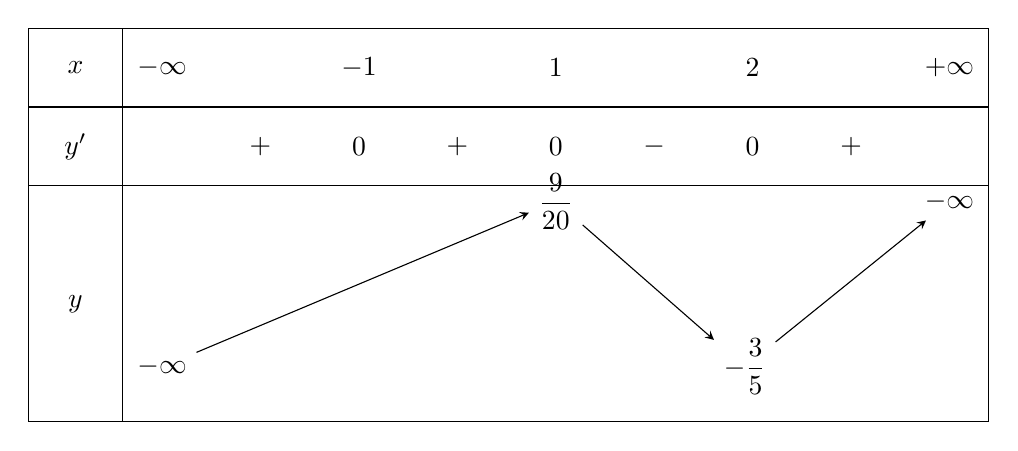
\begin{tikzpicture}[>=stealth]
            \tkzTabInit[nocadre=false,lgt=1.2,espcl=2.5]
            {$x$ / 1, $y'$ / 1, $y$ / 3}
            {$-\infty$, $-1$, $1$,$2$, $+\infty$}
            \tkzTabLine{ , +, 0, +, 0, -,0,+ }
            
            
            \node (y1) at (1.7, -4.3) {$-\infty$};
            \node (y2) at (6.7, -2.2) {$\dfrac{9}{20}$};
            \node (y3) at (9.1, -4.3) {$-\dfrac{3}{5}$};
            \node (y4) at (11.7, -2.2) {$-\infty$};
            
            \draw[->] (y1) -- (y2);
            \draw[->] (y2) -- (y3);
            \draw[->] (y3) -- (y4);
        \end{tikzpicture}
\end{center}

}{
    \textbf{a)} & Hàm số đồng biến trên khoảng \((-\infty; 1)\).
    & \textcolor{amberorange}{$\bigcirc$} & \textcolor{amberorange}{$\bigcirc$} \\ \hline
    
    \textbf{b)} & Hàm số đạt cực đại tại \(x = 1\) và đạt cực tiểu tại \(x = 2\).
    & \textcolor{amberorange}{$\bigcirc$} & \textcolor{amberorange}{$\bigcirc$} \\ \hline
    
    \textbf{c)} & Hàm số có 3 cực trị.
    & \textcolor{amberorange}{$\bigcirc$} & \textcolor{amberorange}{$\bigcirc$} \\ \hline
    
    \textbf{d)} & Hàm số có giá trị lớn nhất bằng \(\dfrac{9}{20}\) và giá trị nhỏ nhất bằng \(-\dfrac{3}{5}\).
    & \textcolor{amberorange}{$\bigcirc$} & \textcolor{amberorange}{$\bigcirc$} \\
}

% --- CÂU 70: BẢNG BIẾN THIÊN ---
\questionTrueFalse{0}{70}{Cho hàm số \( y = f(x) \) có bảng biến thiên như hình vẽ.

\begin{center}
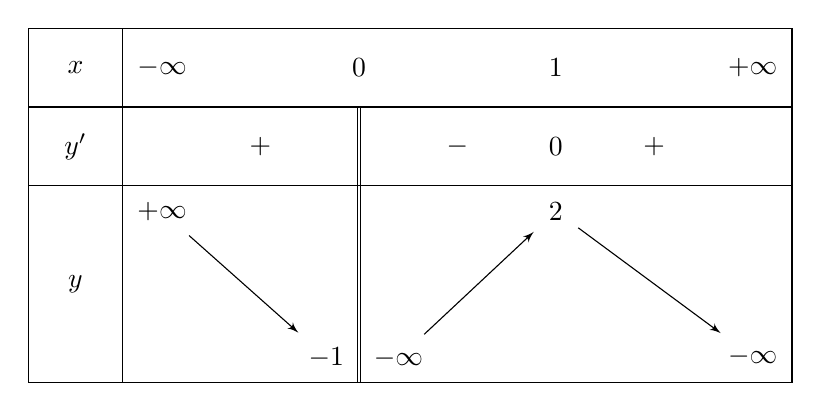
\begin{tikzpicture}[>=stealth]
    \tkzTabInit[nocadre=false, lgt=1.2, espcl=2.5]
        {$x$ / 1, $y'$ / 1, $y$ / 2.5}
        {$-\infty$, $0$, $1$, $+\infty$}
    
    % Sử dụng d để tạo vạch đứng đơn tại vị trí số 0
    \tkzTabLine{ , +, d, -, 0, + }
    
    \tkzTabVar{+/ $+\infty$, -D-/ $-1$ / $-\infty$, +/ $2$, -/ $-\infty$}
\end{tikzpicture}
\end{center}

Xét tính đúng sai của các mệnh đề sau}{
    \textbf{a)} & Hàm số đã cho có hai điểm cực trị.
    & \textcolor{amberorange}{$\bigcirc$} & \textcolor{amberorange}{$\bigcirc$} \\ \hline
    
    \textbf{b)} & \(\min\limits_{(-\infty; 0]} f(x) = -1\).
    & \textcolor{amberorange}{$\bigcirc$} & \textcolor{amberorange}{$\bigcirc$} \\ \hline
    
    \textbf{c)} & \(\max\limits_{(0; +\infty)} f(x) = 2\).
    & \textcolor{amberorange}{$\bigcirc$} & \textcolor{amberorange}{$\bigcirc$} \\ \hline
    
    \textbf{d)} & \(\max\limits_{\mathbb{R} \setminus \{0\}} f(x) = 2\).
    & \textcolor{amberorange}{$\bigcirc$} & \textcolor{amberorange}{$\bigcirc$} \\
}

% --- CÂU 71: BẢNG BIẾN THIÊN CÓ TIỆM CẬN ---
\questionTrueFalse{0}{71}{Cho hàm số \( y = f(x) \) xác định, liên tục trên \( D = \mathbb{R} \setminus \{-1\} \) và có bảng biến thiên như hình vẽ.

\begin{center}
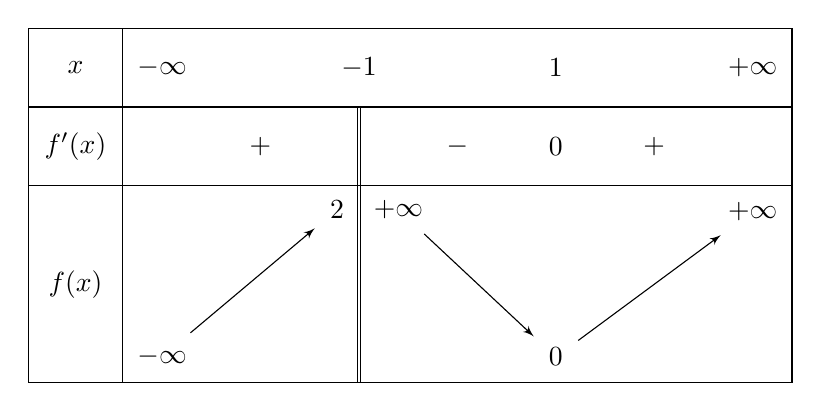
\begin{tikzpicture}[>=stealth]
    \tkzTabInit[nocadre=false, lgt=1.2, espcl=2.5]
        {$x$ / 1, $f'(x)$ / 1, $f(x)$ / 2.5}
        {$-\infty$, $-1$, $1$, $+\infty$}
    
    % Cần đúng số ký tự: 7 ký tự cho 4 cột
    \tkzTabLine{ , +, d, -, 0, +, }
    
    % Cần 5 giá trị cho 4 cột
    \tkzTabVar{-/ $-\infty$,+D+/ $2$ / $+\infty$,-/ $0$, +/ $+\infty$}
\end{tikzpicture}
\end{center}

Xét tính đúng sai của các mệnh đề sau}{
    \textbf{a)} & Hàm số đã cho đạt cực tiểu tại \( x = 1 \).
    & \textcolor{amberorange}{$\bigcirc$} & \textcolor{amberorange}{$\bigcirc$} \\ \hline
    
    \textbf{b)} & Hàm số đã cho đạt cực đại tại điểm \( x = -1 \).
    & \textcolor{amberorange}{$\bigcirc$} & \textcolor{amberorange}{$\bigcirc$} \\ \hline
    
    \textbf{c)} & \(\max\limits_D f(x) = 2\).
    & \textcolor{amberorange}{$\bigcirc$} & \textcolor{amberorange}{$\bigcirc$} \\ \hline
    
    \textbf{d)} & \(\min\limits_{(-1; +\infty)} f(x) = 0\).
    & \textcolor{amberorange}{$\bigcirc$} & \textcolor{amberorange}{$\bigcirc$} \\
}

% --- CÂU 72: HÀM SỐ BẬC 3 ---
\questionTrueFalse{0}{72}{Cho hàm số \( y = f(x) = x^3 - 3x^2 - 9x + 35 \). Xét tính đúng sai của các mệnh đề sau}{
    \textbf{a)} & \(\max\limits_{[-4;4]} f(x) = 40\) đạt được khi \( x = -1 \).
    & \textcolor{amberorange}{$\bigcirc$} & \textcolor{amberorange}{$\bigcirc$} \\ \hline
    
    \textbf{b)} & \(\min\limits_{[-4;4]} f(x) = 8\) đạt được khi \( x = 3 \).
    & \textcolor{amberorange}{$\bigcirc$} & \textcolor{amberorange}{$\bigcirc$} \\ \hline
    
    \textbf{c)} & Hàm số đã cho không có giá trị lớn nhất trên \( \mathbb{R} \).
    & \textcolor{amberorange}{$\bigcirc$} & \textcolor{amberorange}{$\bigcirc$} \\ \hline
    
    \textbf{d)} & Giá trị cực tiểu của \( f(x) \) bằng 8.
    & \textcolor{amberorange}{$\bigcirc$} & \textcolor{amberorange}{$\bigcirc$} \\
}

% --- CÂU 73: HÀM SỐ BẬC 4 TRÙNG PHƯƠNG ---
\questionTrueFalse{0}{73}{Cho hàm số \( f(x) = x^4 - 2x^2 - 15 \). Xét tính đúng sai của các mệnh đề sau}{
    \textbf{a)} & \(\min\limits_{[-2;3]} f(x) = -16\).
    & \textcolor{amberorange}{$\bigcirc$} & \textcolor{amberorange}{$\bigcirc$} \\ \hline
    
    \textbf{b)} & Hàm số đã cho có ba điểm cực trị.
    & \textcolor{amberorange}{$\bigcirc$} & \textcolor{amberorange}{$\bigcirc$} \\ \hline
    
    \textbf{c)} & \(\max\limits_{[-2;3]} f(x) = 8\).
    & \textcolor{amberorange}{$\bigcirc$} & \textcolor{amberorange}{$\bigcirc$} \\ \hline
    
    \textbf{d)} & Hàm số \( f(x) \) không có giá trị nhỏ nhất trên tập số thực.
    & \textcolor{amberorange}{$\bigcirc$} & \textcolor{amberorange}{$\bigcirc$} \\
}

% --- CÂU 74: HÀM SỐ PHÂN THỨC ---
\questionTrueFalse{0}{74}{Cho hàm số \( f(x) = \dfrac{x^2 + x + 2}{x + 2} \). Xét tính đúng sai của các mệnh đề sau}{
    \textbf{a)} & Hàm số \( f(x) \) đồng biến trên mỗi khoảng xác định.
    & \textcolor{amberorange}{$\bigcirc$} & \textcolor{amberorange}{$\bigcirc$} \\ \hline
    
    \textbf{b)} & Hàm số \( f(x) \) có hai điểm cực trị.
    & \textcolor{amberorange}{$\bigcirc$} & \textcolor{amberorange}{$\bigcirc$} \\ \hline
    
    \textbf{c)} & Giá trị lớn nhất của hàm số bằng -7.
    & \textcolor{amberorange}{$\bigcirc$} & \textcolor{amberorange}{$\bigcirc$} \\ \hline
    
    \textbf{d)} & Hàm số \( f(x) \) không có giá trị lớn nhất và giá trị nhỏ nhất trên tập xác định của nó.
    & \textcolor{amberorange}{$\bigcirc$} & \textcolor{amberorange}{$\bigcirc$} \\
}

% --- CÂU 75: ĐỒ THỊ f'(x) TRÊN ĐOẠN [-2; 2] ---
\questionTrueFalse{0}{75}{Cho hàm số \( y = f(x) \). Đồ thị hàm số \( y = f'(x) \) trên đoạn \([-2; 2]\) là đường cong trong hình vẽ.

\begin{center}
\begin{tikzpicture}[>=latex, scale=1.3]
    % 1. Hệ trục tọa độ Ox, Oy màu đen
    \draw[->, black, thick] (-2.8, 0) -- (2.8, 0) node[below] {\small $x$};
    \draw[->, black, thick] (0, -1.8) -- (0, 3.5) node[right] {\small $y$};
    \node[below left] at (0,0) {\small $O$};
    
    % 2. Đồ thị hàm số màu tím (Purple)
    % Đường cong giảm mượt mà từ (-2, 2.8) qua trục Oy, cắt Ox tại (1,0) và dừng ở (2,-1)
    \draw[purple, thick] (-2, 2.8) to[out=-55, in=155] (0, 0.4) 
                                 to[out=-25, in=140] (1, 0) 
                                 to[out=-40, in=115] (2, -1);

    % 3. Các đường nét đứt và nhãn tọa độ màu đen
    % Tại x = -2 (Điểm mút trên)
    \draw[dashed, black] (-2, 0) -- (-2, 2.8) -- (0, 2.8);
    \node[below] at (-2, 0) {\small $-2$};
    
    % Tại x = 1 (Giao điểm với trục hoành)
    \node[above] at (1, 0) {\small $1$};
    
    % Tại x = 2 (Điểm mút dưới)
    \draw[dashed, black] (2, 0) -- (2, -1) -- (0, -1);
    \node[above] at (2, 0) {\small $2$};

    % 4. Các điểm chấm tròn đen tại các tọa độ đặc biệt
    \fill[black] (-2, 2.8) circle (1.5pt);
    \fill[black] (1, 0) circle (1.5pt);
    \fill[black] (2, -1) circle (1.5pt);

\end{tikzpicture}
\end{center}

Biết rằng \( f(-1) + f(2) = f(1) + f(-2) \). Xét tính đúng sai của các mệnh đề sau:}{
    \textbf{a)} & \(\max\limits_{[-2;2]} f(x) = f(-2)\).
    & \textcolor{amberorange}{$\bigcirc$} & \textcolor{amberorange}{$\bigcirc$} \\ \hline
    
    \textbf{b)} & \(\max\limits_{[-2;2]} f(x) = f(1)\).
    & \textcolor{amberorange}{$\bigcirc$} & \textcolor{amberorange}{$\bigcirc$} \\ \hline
    
    \textbf{c)} & \( f(1) < f(0) < f(-2) \).
    & \textcolor{amberorange}{$\bigcirc$} & \textcolor{amberorange}{$\bigcirc$} \\ \hline
    
    \textbf{d)} & \(\min\limits_{[-2;2]} f(x) = f(-2)\).
    & \textcolor{amberorange}{$\bigcirc$} & \textcolor{amberorange}{$\bigcirc$} \\
}

% --- CÂU 76: ĐỒ THỊ f'(x) TRÊN ĐOẠN [-3; 3] ---
\questionTrueFalse{0}{76}{Cho hàm số \( y = f(x) \). Đồ thị hàm số \( y = f'(x) \) trên đoạn \([-3; 3]\) là đường cong trong hình vẽ.

\begin{center}
\begin{tikzpicture}[>=latex, xscale=1.2, yscale=0.8]
    % 1. Hệ trục tọa độ Ox, Oy màu đen
    \draw[->, black, thick] (-4.0, 0) -- (4.2, 0) node[above] {\small $x$};
    \draw[->, black, thick] (0, -5.0) -- (0, 3.8) node[right] {\small $y$};
    \node[below left] at (0,0) {\small $O$};
    
    % 2. Các đường nét đứt và nhãn tọa độ màu đen
    % Tại x = -3, y = -4
    \draw[dashed, black] (-3, 0) -- (-3, -4) -- (0, -4);
    \node[above] at (-3, 0) {\small $-3$};
    \node[right] at (0, -4) {\small $-4$};
    
    % Tại vị trí x = 1 (Giao điểm đồ thị với Ox)
    \node[below right] at (1, 0) {\small $1$};
    
    % Tại x = 3, y = 2
    \draw[dashed, black] (3, 0) -- (3, 2) -- (0, 2);
    \node[below] at (3, 0) {\small $3$};
    \node[left] at (0, 2) {\small $2$};
    
    % 3. Đồ thị hàm số uốn lượn màu tím (Purple)
    % Đồ thị đi qua (-3, -4), lên cực đại, xuống cực tiểu, cắt Oy, qua (1,0), uốn nhẹ rồi qua (3,2)
    \draw[purple, thick] 
        (-3.2, -5.0) .. controls (-3.1, -4.5) .. (-3, -4) 
                     to[out=75, in=180] (-2.1, -1.3) 
                     to[out=0, in=180] (-1.1, -2.2) 
                     to[out=0, in=220] (1, 0) 
                     to[out=40, in=180] (2.0, 0.4) 
                     to[out=0, in=250] (3, 2) 
                     .. controls (3.1, 2.7) .. (3.3, 3.6);

\end{tikzpicture}
\end{center}

Biết rằng \( f(-3) + 2f(1) = f(3) + 2f(0) \). Xét tính đúng sai của các mệnh đề sau:}{
    \textbf{a)} & \(\min\limits_{[-3;3]} f(x) = f(-3) = -4\).
    & \textcolor{amberorange}{$\bigcirc$} & \textcolor{amberorange}{$\bigcirc$} \\ \hline
    
    \textbf{b)} & \(\min\limits_{[-3;3]} f(x) = f(1)\).
    & \textcolor{amberorange}{$\bigcirc$} & \textcolor{amberorange}{$\bigcirc$} \\ \hline
    
    \textbf{c)} & \(\max\limits_{[-3;3]} f(x) = f(-3)\).
    & \textcolor{amberorange}{$\bigcirc$} & \textcolor{amberorange}{$\bigcirc$} \\ \hline
    
    \textbf{d)} & \(\max\limits_{[-3;3]} f(x) = f(3)\).
    & \textcolor{amberorange}{$\bigcirc$} & \textcolor{amberorange}{$\bigcirc$} \\
}

% --- CÂU 77: HÀM SỐ PHÂN THỨC ---
\questionTrueFalse{0}{77}{Cho hàm số \( f(x) = \dfrac{x}{x^2 + 1} \). Xét tính đúng sai của các mệnh đề sau}{
    \textbf{a)} & Đạo hàm của hàm số đã cho là \( f'(x) = \dfrac{x^2 - 1}{(x^2 + 1)^2} \).
    & \textcolor{amberorange}{$\bigcirc$} & \textcolor{amberorange}{$\bigcirc$} \\ \hline
    
    \textbf{b)} & \( x = 1 \) là điểm cực tiểu của hàm số.
    & \textcolor{amberorange}{$\bigcirc$} & \textcolor{amberorange}{$\bigcirc$} \\ \hline
    
    \textbf{c)} & Hàm số có hai điểm cực trị.
    & \textcolor{amberorange}{$\bigcirc$} & \textcolor{amberorange}{$\bigcirc$} \\ \hline
    
    \textbf{d)} & Hàm số có giá trị nhỏ nhất bằng \(-\dfrac{1}{2}\).
    & \textcolor{amberorange}{$\bigcirc$} & \textcolor{amberorange}{$\bigcirc$} \\
}

% --- CÂU 78: ĐỒ THỊ HÀM SỐ ---
\questionTrueFalse{0}{78}{ Cho đồ thị hàm số \( y = f(x) \) có hình vẽ dưới đây và có tập xác định trên \( \mathbb{R} \).

\begin{center}
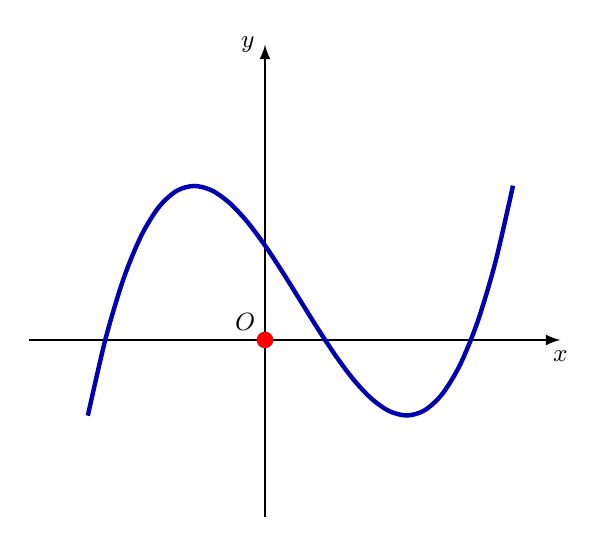
\begin{tikzpicture}[>=latex, scale=1.5]
    % 1. Hệ trục tọa độ Ox, Oy màu đen
    \draw[->, black, thick] (-2, 0) -- (2.5, 0) node[below] {\small $x$};
    \draw[->, black, thick] (0, -1.5) -- (0, 2.5) node[left] {\small $y$};
    \node[above left] at (0,0) {\small $O$};
    
    % 2. Đồ thị hàm số màu xanh dương (gần giống nguyên bản)
    % Sử dụng hàm số bậc ba mô phỏng chính xác dáng điệu của hình: y = 0.67*x^3 - 0.6*x^2 - 1.44*x + 0.8
    \draw[blue!70!black, ultra thick, smooth, domain=-1.5:2.1] 
        plot (\x, {0.667*(\x)^3 - 0.6*(\x)^2 - 1.44*(\x) + 0.8});

    % 3. Chấm tròn màu đỏ tại gốc tọa độ O theo đúng ảnh gốc
    \fill[red] (0,0) circle (2pt);

\end{tikzpicture}
\end{center}

}{
    \textbf{a)} & Đồ thị hàm số đã cho là của hàm số \( y = \dfrac{2x^2 - 1}{x + 1} \).
    & \textcolor{amberorange}{$\bigcirc$} & \textcolor{amberorange}{$\bigcirc$} \\ \hline
    
    \textbf{b)} & Hàm số đã cho không có giá trị lớn nhất và nhỏ nhất.
    & \textcolor{amberorange}{$\bigcirc$} & \textcolor{amberorange}{$\bigcirc$} \\ \hline
    
    \textbf{c)} & Hàm số có đồ thị đã cho đồng biến trên \( \mathbb{R} \).
    & \textcolor{amberorange}{$\bigcirc$} & \textcolor{amberorange}{$\bigcirc$} \\ \hline
    
    \textbf{d)} & Đồ thị hàm số đã cho có hai cực trị.
    & \textcolor{amberorange}{$\bigcirc$} & \textcolor{amberorange}{$\bigcirc$} \\
}

% --- CÂU 79: ĐỒ THỊ f'(x) ---
\questionTrueFalse{0}{79}{ Cho hàm số \( y = f(x) \) có đạo hàm liên tục trên \( \mathbb{R} \). Hàm số \( y = f'(x) \) có đồ thị như hình dưới đây.

\begin{center}
\begin{tikzpicture}[>=latex, scale=1.2]
    % 1. Hệ trục tọa độ Ox, Oy màu xám đậm
    \draw[->, black!70, thick] (-2.2, 0) -- (5.2, 0) node[below] {\small $x$};
    \draw[->, black!70, thick] (0, -2.5) -- (0, 3.2) node[left] {\small $y$};
    \node[below left] at (0,0) {\small $0$};
    
    % 2. Các nhãn tọa độ trên trục hoành Ox
    \node[below right] at (-1, 0) {\small $-1$};
    \node[above right] at (1, 0) {\small $1$};
    \node[below right] at (4, 0) {\small $4$};
    
    % 3. Đồ thị hàm số bậc ba (màu xám đen, nét dày)
    % Công thức mô phỏng chính xác tỉ lệ: y = 0.22 * (x + 1) * (x - 1) * (x - 4)
    \draw[black!80, ultra thick, smooth, domain=-1.6:4.6] 
        plot (\x, {0.22*(\x+1)*(\x-1)*(\x-4)});

\end{tikzpicture}
\end{center}

}{
    \textbf{a)} & Hàm số \( y = f(x) \) đồng biến trên khoảng \( (1; +\infty) \).
    & \textcolor{amberorange}{$\bigcirc$} & \textcolor{amberorange}{$\bigcirc$} \\ \hline
    
    \textbf{b)} & Trên đoạn \([-1; 4]\) thì giá trị lớn nhất của hàm số \( y = f(x) \) là \( f(1) \).
    & \textcolor{amberorange}{$\bigcirc$} & \textcolor{amberorange}{$\bigcirc$} \\ \hline
    
    \textbf{c)} & \( f(1) > f(2) > f(4) \).
    & \textcolor{amberorange}{$\bigcirc$} & \textcolor{amberorange}{$\bigcirc$} \\ \hline
    
    \textbf{d)} & Hàm số \( y = f(x) \) có hai cực trị.
    & \textcolor{amberorange}{$\bigcirc$} & \textcolor{amberorange}{$\bigcirc$} \\
}

% --- CÂU 80: HÀM SỐ LƯỢNG GIÁC ---
\questionTrueFalse{0}{80}{Cho hàm số \( f(x) = 4 \sin x \cos x + 2x \).}{
    \textbf{a)} & Đạo hàm của hàm số đã cho là \( f'(x) = 4 \sin 2x + 2 \).
    & \textcolor{amberorange}{$\bigcirc$} & \textcolor{amberorange}{$\bigcirc$} \\ \hline
    
    \textbf{b)} & Hàm số \( y = f(x) \) có 4 điểm cực trị thuộc \([- \pi; \pi]\).
    & \textcolor{amberorange}{$\bigcirc$} & \textcolor{amberorange}{$\bigcirc$} \\ \hline
    
    \textbf{c)} & Hàm số \( y = f(x) \) đồng biến trên khoảng \((-2; -1)\).
    & \textcolor{amberorange}{$\bigcirc$} & \textcolor{amberorange}{$\bigcirc$} \\ \hline
    
    \textbf{d)} & Giá trị lớn nhất của \( f(x) \) trên đoạn \( \left[0; \dfrac{\pi}{2}\right] \) là \( \dfrac{2\pi}{3} + \sqrt{3} \).
    & \textcolor{amberorange}{$\bigcirc$} & \textcolor{amberorange}{$\bigcirc$} \\
}

% --- CÂU 81: HÀM SỐ LƯỢNG GIÁC ---
\questionTrueFalse{0}{81}{ Cho hàm số \( f(x) = 2 \cos x + x \).}{
    \textbf{a)} & \( f(0) = 2 \); \( f\left(\dfrac{\pi}{2}\right) = \dfrac{\pi}{2} \).
    & \textcolor{amberorange}{$\bigcirc$} & \textcolor{amberorange}{$\bigcirc$} \\ \hline
    
    \textbf{b)} & Đạo hàm của hàm số đã cho là \( f'(x) = 2 \sin x + 1 \).
    & \textcolor{amberorange}{$\bigcirc$} & \textcolor{amberorange}{$\bigcirc$} \\ \hline
    
    \textbf{c)} & Nghiệm của phương trình \( f'(x) = 0 \) trên đoạn \( \left[ 0; \dfrac{\pi}{2} \right] \) là \( \dfrac{\pi}{6} \).
    & \textcolor{amberorange}{$\bigcirc$} & \textcolor{amberorange}{$\bigcirc$} \\ \hline
    
    \textbf{d)} & Giá trị lớn nhất của \( f(x) \) trên đoạn \( \left[ 0; \dfrac{\pi}{2} \right] \) là \( \dfrac{\pi}{6} + \sqrt{3} \).
    & \textcolor{amberorange}{$\bigcirc$} & \textcolor{amberorange}{$\bigcirc$} \\
}

% --- CÂU 82: HÀM SỐ LƯỢNG GIÁC ---
\questionTrueFalse{0}{82}{ Cho hàm số \( f(x) = \sin x - x \).}{
    \textbf{a)} & Đạo hàm của hàm số đã cho là \( f'(x) = \cos x - 1 \).
    & \textcolor{amberorange}{$\bigcirc$} & \textcolor{amberorange}{$\bigcirc$} \\ \hline
    
    \textbf{b)} & Nghiệm của phương trình \( f'(x) = 0 \) trên đoạn \( \left[ \dfrac{\pi}{2}; \dfrac{3\pi}{2} \right] \) là \( \pi \).
    & \textcolor{amberorange}{$\bigcirc$} & \textcolor{amberorange}{$\bigcirc$} \\ \hline
    
    \textbf{c)} & Giá trị nhỏ nhất của \( f(x) \) trên đoạn \( \left[ \dfrac{\pi}{2}; \dfrac{3\pi}{2} \right] \) là \( -1 - \dfrac{3\pi}{2} \).
    & \textcolor{amberorange}{$\bigcirc$} & \textcolor{amberorange}{$\bigcirc$} \\ \hline
    
    \textbf{d)} & \( f(0) = 0 \); \( f(\pi) = -\pi \).
    & \textcolor{amberorange}{$\bigcirc$} & \textcolor{amberorange}{$\bigcirc$} \\
}

% --- CÂU 83: HÀM SỐ LƯỢNG GIÁC ---
\questionTrueFalse{0}{83}{Cho hàm số \( f(x) = 2\sin x - \sqrt{3}x \).}{
    \textbf{a)} & Một nghiệm của phương trình \( f'(x) = 0 \) là \( x = -\dfrac{\pi}{3} \).
    & \textcolor{amberorange}{$\bigcirc$} & \textcolor{amberorange}{$\bigcirc$} \\ \hline
    
    \textbf{b)} & \( f\left(\dfrac{\pi}{2}\right) = -\dfrac{\pi\sqrt{3}}{2} \).
    & \textcolor{amberorange}{$\bigcirc$} & \textcolor{amberorange}{$\bigcirc$} \\ \hline
    
    \textbf{c)} & Đạo hàm của hàm số là \( f'(x) = 2\cos x - \sqrt{3}, \forall x \in \mathbb{R} \).
    & \textcolor{amberorange}{$\bigcirc$} & \textcolor{amberorange}{$\bigcirc$} \\ \hline
    
    \textbf{d)} & Tổng các nghiệm của phương trình \( f'(x) = 0 \) trong đoạn \( \left[ 0; \dfrac{5\pi}{2} \right] \) bằng \( \dfrac{25\pi}{6} \).
    & \textcolor{amberorange}{$\bigcirc$} & \textcolor{amberorange}{$\bigcirc$} \\
}

% --- CÂU 84: HÀM SỐ BẬC 3 ---
\questionTrueFalse{0}{84}{Cho hàm số \( y = 2x^3 - 3x^2 + 2025 = f(x) \). Các mệnh đề sau đúng hay sai?}{
    \textbf{a)} & Hàm số đã cho có giá trị lớn nhất, nhỏ nhất trên \([-2; 0]\).
    & \textcolor{amberorange}{$\bigcirc$} & \textcolor{amberorange}{$\bigcirc$} \\ \hline
    
    \textbf{b)} & Gọi \( M, m \) lần lượt là giá trị lớn nhất, giá trị nhỏ nhất của hàm số \( f(x) \) trên đoạn \([0; 1]\). Khi đó \( M + m = 2024 \).
    & \textcolor{amberorange}{$\bigcirc$} & \textcolor{amberorange}{$\bigcirc$} \\ \hline
    
    \textbf{c)} & Hàm số đạt giá trị nhỏ nhất trên \([0; +\infty)\) tại \( x = 1 \).
    & \textcolor{amberorange}{$\bigcirc$} & \textcolor{amberorange}{$\bigcirc$} \\ \hline
    
    \textbf{d)} & Có 20 giá trị nguyên của \( k \in [-2025; 2025] \) để phương trình \( 2x^3 - 3x^2 + 2k - 1 = 0 \) có 3 nghiệm phân biệt trên \([-1; 3]\).
    & \textcolor{amberorange}{$\bigcirc$} & \textcolor{amberorange}{$\bigcirc$} \\
}

% --- CÂU 85: HÀM SỐ PHÂN THỨC ---
\questionTrueFalse{0}{85}{Cho hàm số \( y = \dfrac{x^2 - x + 1}{x - 1} = f(x) \). Các mệnh đề sau đúng hay sai?}{
    \textbf{a)} & Hàm số đã cho có giá trị lớn nhất, nhỏ nhất trên \([0; 2]\).
    & \textcolor{amberorange}{$\bigcirc$} & \textcolor{amberorange}{$\bigcirc$} \\ \hline
    
    \textbf{b)} & Gọi \( M, m \) lần lượt là giá trị lớn nhất, giá trị nhỏ nhất của hàm số \( f(x) \) trên \([-1; 0]\). Khi đó \( M + 2m = -4 \).
    & \textcolor{amberorange}{$\bigcirc$} & \textcolor{amberorange}{$\bigcirc$} \\ \hline
    
    \textbf{c)} & Hàm số đạt giá trị lớn nhất trên \((1; +\infty)\) tại \( x = 2 \).
    & \textcolor{amberorange}{$\bigcirc$} & \textcolor{amberorange}{$\bigcirc$} \\ \hline
    
    \textbf{d)} & Có 2026 giá trị nguyên của \( k \in [-2025; 2025] \) để bất phương trình \( 2a - \dfrac{x^2 - x + 1}{x - 1} \geq 0 \) nghiệm đúng \( \forall x \in (-\infty; 1) \).
    & \textcolor{amberorange}{$\bigcirc$} & \textcolor{amberorange}{$\bigcirc$} \\
}

% --- CÂU 86: HÀM SỐ PHÂN THỨC ---
\questionTrueFalse{0}{86}{Cho hàm số \( y = f(x) = \dfrac{2x - 1}{x - 3} \).}{
    \textbf{a)} & \( y' = \dfrac{-5}{(x - 3)^2}, \forall x \neq 3 \).
    & \textcolor{amberorange}{$\bigcirc$} & \textcolor{amberorange}{$\bigcirc$} \\ \hline
    
    \textbf{b)} & \( f(-2) = 3; f(1) = -2 \).
    & \textcolor{amberorange}{$\bigcirc$} & \textcolor{amberorange}{$\bigcirc$} \\ \hline
    
    \textbf{c)} & Giá trị lớn nhất và giá trị nhỏ nhất của hàm số \( f(x) \) trên đoạn \([-2; 1]\) lần lượt là \( 1; -\dfrac{1}{2} \).
    & \textcolor{amberorange}{$\bigcirc$} & \textcolor{amberorange}{$\bigcirc$} \\ \hline
    
    \textbf{d)} & Hàm số \( y = f(x) \) đạt giá trị lớn nhất trên đoạn \([-1; 2]\) tại \( x_0 = -1 \).
    & \textcolor{amberorange}{$\bigcirc$} & \textcolor{amberorange}{$\bigcirc$} \\
}

% --- CÂU 87: HÀM SỐ LOGARIT ---
\questionTrueFalse{0}{87}{Cho hàm số \( y = x - \ln x \).}{
    \textbf{a)} & Tập xác định của hàm số là \( D = \mathbb{R} \).
    & \textcolor{amberorange}{$\bigcirc$} & \textcolor{amberorange}{$\bigcirc$} \\ \hline
    
    \textbf{b)} & Đạo hàm của hàm số là \( y' = 1 - \dfrac{1}{x} \).
    & \textcolor{amberorange}{$\bigcirc$} & \textcolor{amberorange}{$\bigcirc$} \\ \hline
    
    \textbf{c)} & Giá trị nhỏ nhất của hàm số trên đoạn \( \left[\dfrac{1}{2}; e\right] \) bằng 1.
    & \textcolor{amberorange}{$\bigcirc$} & \textcolor{amberorange}{$\bigcirc$} \\ \hline
    
    \textbf{d)} & Giá trị lớn nhất của hàm số trên đoạn \( \left[\dfrac{1}{2}; e\right] \) bằng \( \dfrac{1}{2} + \ln 2 \).
    & \textcolor{amberorange}{$\bigcirc$} & \textcolor{amberorange}{$\bigcirc$} \\
}

% --- CÂU 88: HÀM SỐ LOGARIT ---
\questionTrueFalse{0}{88}{Cho hàm số \( y = \log_3(x^2 - 2x) \).}{
    \textbf{a)} & Tập xác định của hàm số là \( D = (-\infty; 0) \cup (2; +\infty) \).
    & \textcolor{amberorange}{$\bigcirc$} & \textcolor{amberorange}{$\bigcirc$} \\ \hline
    
    \textbf{b)} & Đạo hàm của hàm số là \( y' = \dfrac{2x - 2}{(x^2 - 2x)\ln 3} \).
    & \textcolor{amberorange}{$\bigcirc$} & \textcolor{amberorange}{$\bigcirc$} \\ \hline
    
    \textbf{c)} & Giá trị nhỏ nhất của hàm số trên đoạn \([3; 5]\) bằng 1.
    & \textcolor{amberorange}{$\bigcirc$} & \textcolor{amberorange}{$\bigcirc$} \\ \hline
    
    \textbf{d)} & Giá trị lớn nhất của hàm số trên đoạn \([-3; -1]\) bằng \( \log_3 5 \).
    & \textcolor{amberorange}{$\bigcirc$} & \textcolor{amberorange}{$\bigcirc$} \\
}

% --- CÂU 89: HÀM SỐ LOGARIT ---
\questionTrueFalse{0}{89}{(Sở Vĩnh Phúc 2025) Cho hàm số \( f(x) = 2x - \log_5(x + 1) \).}{
    \textbf{a)} & Đạo hàm của hàm số \( f(x) \) là \( f'(x) = 1 - \dfrac{1}{x + 1}, \forall x \in (-1; +\infty) \).
    & \textcolor{amberorange}{$\bigcirc$} & \textcolor{amberorange}{$\bigcirc$} \\ \hline
    
    \textbf{b)} & Hàm số \( f(x) \) có một điểm cực tiểu.
    & \textcolor{amberorange}{$\bigcirc$} & \textcolor{amberorange}{$\bigcirc$} \\ \hline
    
    \textbf{c)} & Giá trị của hàm số \( f(x) \) tại điểm \( x = 4 \) là \( f(4) = 8 \).
    & \textcolor{amberorange}{$\bigcirc$} & \textcolor{amberorange}{$\bigcirc$} \\ \hline
    
    \textbf{d)} & Hàm số đồng biến trên khoảng \( (0; +\infty) \).
    & \textcolor{amberorange}{$\bigcirc$} & \textcolor{amberorange}{$\bigcirc$} \\
}

















\end{document}